%%%%%%%%%%%%%%%%%%%%%%%%%%%%%%%%%%%%%%%%%
% Arsclassica Article
% LaTeX Template
% Version 1.1 (10/6/14)
%
% This template has been downloaded from:
% http://www.LaTeXTemplates.com
%
% Original author:
% Lorenzo Pantieri (http://www.lorenzopantieri.net) with extensive modifications by:
% Vel (vel@latextemplates.com)
%
% License:
% CC BY-NC-SA 3.0 (http://creativecommons.org/licenses/by-nc-sa/3.0/)
% 
%%%%%%%%%%%%%%%%%%%%%%%%%%%%%%%%%%%%%%%%%

%----------------------------------------------------------------------------------------
%	PACKAGES AND OTHER DOCUMENT CONFIGURATIONS
%----------------------------------------------------------------------------------------

\documentclass[
11pt, % Main document font size
a4paper, % Paper type, use 'letterpaper' for US Letter paper
oneside, % One page layout (no page indentation)
%twoside, % Two page layout (page indentation for binding and different headers)
pdfspacing, % Makes use of pdftex’ letter spacing capabilities via the microtype package
headinclude,
%footinclude, % Extra spacing for the header and footer
BCOR5mm, % Binding correction
ngerman, %set document to German
bibtotocnumbered,
]{scrartcl}
%{scrartcl}

%----------------------------------------------------------------------------------------
%	REQUIRED PACKAGES
%----------------------------------------------------------------------------------------

\usepackage{graphicx} % Required for including images
\graphicspath{{Figures/}} % Set the default folder for images

\usepackage[square,
authoryear,
]{natbib}

\usepackage{relsize, etoolbox, lmodern}% http://ctan.org/pkg/{relsize,etoolbox}

\AtBeginEnvironment{quote}{\smaller\fontfamily{lmss}\selectfont}% Step font down one size relative to current font.
% see http://tex.stackexchange.com/questions/25249/how-do-i-use-a-particular-font-for-a-small-section-of-text-in-my-document for fontfamilies

\usepackage{chngcntr}

% to have a separation in the text with extra space between paragraphs and no indendation following
\newcommand*{\skippingparagraph}{\par\vspace{1.0\baselineskip}\noindent}

\usepackage[absolute,overlay]{textpos}

\setbeamercolor{framesource}{fg=gray}
\setbeamerfont{framesource}{size=\tiny}

\newcommand{\source}[1]{\begin{textblock*}{6cm}(6.7cm,8.6cm)
		\begin{beamercolorbox}[ht=0.5cm,right]{framesource}
			\usebeamerfont{framesource}\usebeamercolor[fg]{framesource} Source: {#1}
		\end{beamercolorbox}
\end{textblock*}}

%Framenumber in Header
%http://tex.stackexchange.com/a/145899/123262

\makeatletter
\setbeamertemplate{frametitle}{%
	\nointerlineskip%
	\vskip-\beamer@headheight%
	\vbox to \beamer@headheight{%
		\vfil
		\leftskip=-\beamer@leftmargin%
		\advance\leftskip by0.3cm%
		\rightskip=-\beamer@rightmargin%
		\advance\rightskip by0.3cm plus1fil%
		{\usebeamercolor[fg]{frametitle}
			\usebeamerfont{frametitle}\insertframetitle\par}% added number
		{\usebeamercolor[fg]{framesubtitle}
			\usebeamerfont{framesubtitle}\insertframesubtitle\hfill{\tiny\insertframenumber/\inserttotalframenumber}\par}%
		\vbox{}%
		\vskip-1em%
		\vfil
	}%
}
\makeatother
%----------------------------------------------------------------------------------------
%	HYPERLINKS
%---------------------------------------------------------------------------------------

\hypersetup{
	%draft, % Uncomment to remove all links (useful for printing in black and white)
	colorlinks=true, breaklinks=true, bookmarks=true,bookmarksnumbered,
	urlcolor=brown, linkcolor=blue, citecolor=green, % Link colors
	pdftitle={}, % PDF title
	pdfauthor={\textcopyright}, % PDF Author
	pdfsubject={}, % PDF Subject
	pdfkeywords={}, % PDF Keywords
	pdfcreator={pdfLaTeX}, % PDF Creator
	pdfproducer={LaTeX with hyperref and ClassicThesis} % PDF producer
}


%----------------------------------------------------------------------------------------
%	CODESNIPPETS
%---------------------------------------------------------------------------------------

%%%%%%%%%%%%%%%%%%%%%%%%%%%%%%%%%%%%%%%%%
% Code Snippet
% LaTeX Template
% Version 1.0 (14/2/13)
%
% This template has been downloaded from:
% http://www.LaTeXTemplates.com
%
% Original author:
% Velimir Gayevskiy (vel@latextemplates.com)
%
% License:
% CC BY-NC-SA 3.0 (http://creativecommons.org/licenses/by-nc-sa/3.0/)
%
%%%%%%%%%%%%%%%%%%%%%%%%%%%%%%%%%%%%%%%%%
\usepackage{wasysym}

\usepackage{listings} % Required for inserting code snippets
\usepackage{pgf, pgffor}
\usepackage{lstlinebgrd} % see http://www.ctan.org/pkg/lstaddons

\definecolor{DarkGreen}{rgb}{0.0,0.4,0.0} % Comment color
\definecolor{highlight}{RGB}{255,251,204} % Code highlight color

%%% listingsbackground from http://tex.stackexchange.com/a/85628/123262
\makeatletter
%%%%%%%%%%%%%%%%%%%%%%%%%%%%%%%%%%%%%%%%%%%%%%%%%%%%%%%%%%%%%%%%%%%%%%%%%%%%%%
%
% \btIfInRange{number}{range list}{TRUE}{FALSE}
%
% Test in int number <number> is element of a (comma separated) list of ranges
% (such as: {1,3-5,7,10-12,14}) and processes <TRUE> or <FALSE> respectively

\newcount\bt@rangea
\newcount\bt@rangeb

\newcommand\btIfInRange[2]{%
	\global\let\bt@inrange\@secondoftwo%
	\edef\bt@rangelist{#2}%
	\foreach \range in \bt@rangelist {%
		\afterassignment\bt@getrangeb%
		\bt@rangea=0\range\relax%
		\pgfmathtruncatemacro\result{ ( #1 >= \bt@rangea) && (#1 <= \bt@rangeb) }%
		\ifnum\result=1\relax%
		\breakforeach%
		\global\let\bt@inrange\@firstoftwo%
		\fi%
	}%
	\bt@inrange%
}
\newcommand\bt@getrangeb{%
	\@ifnextchar\relax%
	{\bt@rangeb=\bt@rangea}%
	{\@getrangeb}%
}
\def\@getrangeb-#1\relax{%
	\ifx\relax#1\relax%
	\bt@rangeb=100000%   \maxdimen is too large for pgfmath
	\else%
	\bt@rangeb=#1\relax%
	\fi%
}

%%%%%%%%%%%%%%%%%%%%%%%%%%%%%%%%%%%%%%%%%%%%%%%%%%%%%%%%%%%%%%%%%%%%%%%%%%%%%%
%
% \btLstHL<overlay spec>{range list}
%
% TODO BUG: \btLstHL commands can not yet be accumulated if more than one overlay spec match.
% 
\newcommand<>{\btLstHL}[1]{%
	\only#2{\btIfInRange{\value{lstnumber}}{#1}{\color{orange!30}\def\lst@linebgrdcmd{\color@block}}{\def\lst@linebgrdcmd####1####2####3{}}}%
}%
\makeatother

\lstdefinestyle{JSStyle}{ % Define a style for your code snippet, multiple definitions can be made if, for example, you wish to insert multiple code snippets using different programming languages into one document
	language=JavaScript, % Detects keywords, comments, strings, functions, etc for the language specified
%	backgroundcolor=\color{highlight}, % Set the background color for the snippet - useful for highlighting
	basicstyle=\smaller\smaller\ttfamily, % The default font size and style of the code
	breakatwhitespace=true, % If true, only allows line breaks at white space
%	breaklines=true, % Automatic line breaking (prevents code from protruding outside the box)
	captionpos=b, % Sets the caption position: b for bottom; t for top
	commentstyle=\usefont{T1}{pcr}{m}{sl}\color{DarkGreen}, % Style of comments within the code - dark green courier font
	deletekeywords={}, % If you want to delete any keywords from the current language separate them by commas
	%escapeinside={\%}, % This allows you to escape to LaTeX using the character in the bracket
	firstnumber=1, % Line numbers begin at line 1
%	frame=single, % Frame around the code box, value can be: none, leftline, topline, bottomline, lines, single, shadowbox
%	frameround=tttt, % Rounds the corners of the frame for the top left, top right, bottom left and bottom right positions
	keywordstyle=\color{Blue}\textbf, % Functions are bold and blue
	morekeywords={}, % Add any functions no included by default here separated by commas
	numbers=left, % Location of line numbers, can take the values of: none, left, right
	numbersep=5pt, % Distance of line numbers from the code box
	numberstyle=\tiny\color{Gray}, % Style used for line numbers
	rulecolor=\color{black}, % Frame border color
	showstringspaces=false, % Don't put marks in string spaces
	showtabs=false, % Display tabs in the code as lines
%	stepnumber=5, % The step distance between line numbers, i.e. how often will lines be numbered
	stringstyle=\color{Purple}, % Strings are purple
	tabsize=2, % Number of spaces per tab in the code
}

\definecolor{darkgray}{rgb}{.4,.4,.4}
\definecolor{purple}{rgb}{0.65, 0.12, 0.82}


%define Javascript language
\lstdefinelanguage{JavaScript}{
	keywords={typeof, new, true, false, catch, try, finally, function, return, null, then, catch, switch, var, if, in, while, do, else, case, break, yield, async, await, let, const},
	keywordstyle=\color{blue}\bfseries,
	ndkeywords={class, export, boolean, throw, implements, import, this},
	ndkeywordstyle=\color{darkgray}\bfseries,
	identifierstyle=\color{black},
	sensitive=false,
	comment=[l]{//},
	morecomment=[s]{/*}{*/},
	commentstyle=\color{purple}\ttfamily,
	stringstyle=\color{red}\ttfamily,
	morestring=[b]',
	morestring=[b]"
}

\lstset{
	language=JavaScript,
	extendedchars=true,
	basicstyle=\footnotesize\ttfamily,
	showstringspaces=false,
	showspaces=false,
	numbers=left,
	numberstyle=\footnotesize,
	numbersep=9pt,
	tabsize=2,
	breaklines=true,
	showtabs=false,
	captionpos=b,
	escapeinside={(*@}{@*)},	%see http://tex.stackexchange.com/a/8860/123262
}

% Create a command to cleanly insert a snippet with the style above anywhere in the document
\newcommand{\insertcode}[1]{\lstinputlisting[label=#1,style=JSStyle]{#1}} % The first argument is the script location/filename

 % Include the structure.tex file which specified the document structure and layout

\hyphenation{Fortran hy-phen-ation ECMA-Script Java-Script Prom-ise prom-ise Fremd-co-de Net-scape -Code Code-ab-schnitte Sprach-fea-tures} % Specify custom hyphenation points in words with dashes where you would like hyphenation to occur, or alternatively, don't put any dashes in a word to stop hyphenation altogether

%----------------------------------------------------------------------------------------
%	TITLE AND AUTHOR(S)
%----------------------------------------------------------------------------------------
\selectlanguage{ngerman}
	
\subtitle{\normalfont{Seminar 1908 an der FernUni Hagen im WS 2016/17:\protect\\Moderne Programmiertechniken und -Methoden}}

\title{\normalfont{Asnychrone Programmierung: \protect\\ Moderne Methoden in ECMAScript~6}} % The article title
%\title{\normalfont\spacedallcaps{Asnychrone Programmierung: \protect\\ Moderne Methoden in ECMAScript~6}} % The article title



\author{Felix Eckstein*} % The article author(s) - author affiliations need to be specified in the AUTHOR AFFILIATIONS block

%----------------------------------------------------------------------------------------
%	AUTHOR AFFILIATIONS
%----------------------------------------------------------------------------------------

%\affil[*]{Student im Bachelor of Science Informatik, FernUniversität Hagen, Matr.-\#: 8161569, \href{mailto:felix.eckstein@gmx.de}{felix.eckstein@gmx.de}}


\date{Dezember 2016} % An optional date to appear under the author(s)

%----------------------------------------------------------------------------------------

\begin{document}

	
	
	
%----------------------------------------------------------------------------------------
%	HEADERS
%----------------------------------------------------------------------------------------

\renewcommand{\sectionmark}[1]{\markright{\spacedlowsmallcaps{#1}}} % The header for all pages (oneside) or for even pages (twoside)
%\renewcommand{\subsectionmark}[1]{\markright{\thesubsection~#1}} % Uncomment when using the twoside option - this modifies the header on odd pages
\lehead{\mbox{\llap{\small\thepage\kern1em\color{halfgray} \vline}\color{halfgray}\hspace{0.5em}\rightmark\hfil}} % The header style

\pagestyle{scrheadings} % Enable the headers specified in this block

%----------------------------------------------------------------------------------------
%	TABLE OF CONTENTS & LISTS OF FIGURES AND TABLES
%----------------------------------------------------------------------------------------
\setcounter{page}{1}
\pagenumbering{roman}
\maketitle % Print the title/author/date block

\setcounter{tocdepth}{3} % Set the depth of the table of contents to show sections and subsections only

%----------------------------------------------------------------------------------------
%	ABSTRACT
%----------------------------------------------------------------------------------------
\begin{otherlanguage}{english}
%	\begin{abstract}
		\noindent This paper gives an overview on modern methods of asynchronous programming in the 2015 JavaScript Standard ``ECMAScript~6''. 
		
		Firstly, an overview of the JavaScript runtime environment is given to motivate the excessive use of asynchronous programming in JavaScript applications. The principle of asynchronous programming is briefly introduced. Following this clarification of terms, the traditional callback approach to asynchronous programming is presented together with its inherent downsides.
		
		In the main part of the paper, the modern ECMAScript~6 features ``promises'' and ``generators'' together with their application to asynchronous programming are introduced and discussed in detail. A special focus is laid on the way they solve problems that were present with the traditional callback approach.
		
		The paper concludes with a discussion whether the new language features are worth using and under what circumstances it might be a good option to waive the new features in favor of compatibility to older runtime environments.
		
		The appendix contains examples of common asynchronous patterns in ECMAScript~6.
		
%	\end{abstract}
\end{otherlanguage}

{\let\thefootnote\relax\footnotetext{* \textit{Student im Bachelor of Science Informatik an der FernUniversität Hagen,\protect\\Matr.-\#: 8161569, \href{mailto:felix.eckstein@gmx.de}{felix.eckstein@gmx.de}}}}

\selectlanguage{ngerman}
\cleardoublepage

\tableofcontents % Print the table of contents

\listoffigures % Print the list of figures

\listoftables % Print the list of tables

\lstlistoflistings



%----------------------------------------------------------------------------------------

\cleardoublepage % Start the article content on the second page, remove this if you have a longer abstract that goes onto the second page

%----------------------------------------------------------------------------------------
%	INTRODUCTION
%----------------------------------------------------------------------------------------
\setcounter{page}{1}
\pagenumbering{arabic}
\section{Javascript -- die häufigste Programmiersprache der Welt}


Seit der Erfindung der Sprache "`Mocha"' durch Brendan Eich im Mai 1995 und dem ersten Auftreten dieser inzwischen in JavaScript umbenannten Sprache im Netscape Navigator 2.0 im März 1996 (vgl. \citep{NetscapeSun1995}), hat diese Sprache eine bemerkenswerte Metamorphose erlebt. Zunächst belächelt und relativ nutzlos (vgl. \citep{Buckler2016}) wurde die Sprache stetig weiter entwickelt und schließlich Ende 1996 an die Standardisierungsorganisation ECMA übergeben (vgl.~\citep{NetscapePressRelease.1996})
und im Jahr 1997 im ECMA-262-Standard bzw. ISO/IEC 16262 genormt und offiziell in ECMAScript umbenannt (vgl.~\citep{EcmaTC39.1997}).\footnote{Trotz dieser Umbenennung ist der frühere, noch von Netscape und Sun Microsystems eingeführte Name ein weithin gebrauchtes und übliches Synonym und ein Oberbegriff für die Sprachen, die dieser Spezifikation folgen. Auch in der vorliegenden Arbeit sollen die Begriffe "`ECMAScript", "`ES"', "`JavaScript"' und "`JS"' synonym gebraucht werden. Lediglich wenn es um Features geht, denen speziell der im Jahre 2015 erschienene Standard "`ECMA-262 $6^{\mathrm{th}}$ Edition, The ECMAScript 2015 Language Specification"' zugrunde liegt, wird explizit der Ausdruck "`ES6"' oder "`ECMAScript~6"' benutzt.}
Inzwischen ist Javascript als eine "`echte"' Programmiersprache anerkannt und findet immer stärkere Anwendung. Auch der Einsatzbereich hat sich weit über Scripting im Browser hinaus erweitert, so dass heutzutage insbesondere auch Serverapplikationen häufig in JavaScript realisiert werden.  

\begin{quote}
	The World's Most Misunderstood Programming Language Has Become the World's Most Popular Programming Language~\citep{Crockford.2008a}
\end{quote}

Laut einer Untersuchung der Entwickler-Website "`Stackoverflow"' ist JavaScript inzwischen die am häufigsten nachgefragte Sprache (vgl.\citep{Taft.2016}). Auch das stabile Rankig innerhalb der Top Ten der beliebtesten Programmiersprachen im TIOBE Index und die "`Ehrung"' als "`Programming Language of the Year 2013"' belegen die hohe Popularität der Sprache (vgl. \citep{Tiobe}).

Ein Grund für die Popularität der Sprache dürfte darin liegen, dass sich JavaScript inzwischen als lingua franca des WWW durchgesetzt hat und von jedem aktuellen Browser als clientseitiger Script-Sprache für Webapplikationen unterstützt wird. Da alle aktuellen Browser auch Entwicklerwerkzeuge zum direkten Erstellen, Ausführen und Debuggen von JavaScript Code enthalten, dürfte JavaScript die einzige Programmiersprache sein, für die annähernd jeder Computerbenutzer -- von der Bundeskanzlerin bis zum Computernerd -- eine vollständige Entwicklungsumgebung inklusive Editor, Compiler und Debugger besitzt.

\skippingparagraph    
In JavaScript-Programmen ist asynchrone Programmierung allgegenwärtig. Sie weicht erheblich von dem aus anderen Sprachen gewohnten Programmierpardigma des sequentiellen Programmablaufs mit blockierenden Funktionsaufrufen ab. 

In dieser Arbeit soll daher folgender Frage nachgegangen werden:
Was ist asynchrone Programmierung in JavaScript und welche modernen Methoden zur asynchronen Programmierung bietet der neue Sprachstandard ECMAScript~6?

Es wird zunächst ein kurzer Abriss über die Funktionsweise der Laufzeitumgebung von JavaScript gegeben. Die sich daraus ergebende Notwendigkeit zur asynchronen Programmierung wird erläutert und der Begriff "`asynchrone Programmierung"' skizziert.

Nachfolgend wird erläutert, wie asynchrone Programmierung unter Verwendung von traditionellen Callbacks in Standard-JavaScript vor der Einführung von ECMAScript~6 realisiert wurde. Dabei wird aufgezeigt, welche Nachteile die ausschließliche Verwendung solcher Callbacks für die asynchrone Programmierung mit sich bringt.

Die in ECMAScript~6 neu eingeführten Sprachmittel \emph{Promise} und \emph{Generator} werden detailliert eingeführt und ihre Arbeitsweise erläutert. Dabei werden die Unterschiede dieser neuen Sprachmittel zum traditionellen Ansatz herausgestellt.

Abschließend werden die in ECMAScript~6 neu eingeführten Methoden zur asynchronen Programmierung bewertet um daraus Konsequenzen für deren Einsatz in der Praxis abzuleiten.

In einem Anhang werden Beispiele angegeben, wie typische Muster der asynchronen Programmierung unter Verwendung der ECMAScript~6 Methoden konkret formuliert werden.

\section{Wichtige Eigenschaften von \-JavaScript}

	Zunächst sollen zwei Grundeigenschaften von JavaScript geklärt werden, in denen sie sich deutlich von anderen Sprachen wie z. B. Java und Pascal unterscheidet.\footnote{Das sind die Sprachen, die standardmäßig an der Fernuni Hagen im Informatikstudium gelehrt werden \citep{FernUniHagen.2016}.}
	
	\subsection{Funktionale Eigenschaften}
		
		Eine wichtige Eigenschaft der Sprache sind deren funktionalen Elemente und darunter besonders die Eigenschaft, dass Funktionen als ganz normale Objekte angesehen werden.\footnote{Die ECMAScript~6 Spezifikation hierzu:\begin{quote}
		ECMAScript function objects encapsulate parameterized ECMAScript code closed over a lexical environment and support the dynamic evaluation of that code. An ECMAScript function object is an ordinary object and has the same internal slots and the same internal methods as other ordinary objects.~\citep[~{\S}9.2]{EcmaTC39.}\end{quote}} 	
		
		Funktionen sind damit sogenannte "`First-Class-Citizens"' der Sprache und können daher an Variablen zugewiesen werden, an andere Funktionen als Parameter übergeben werden und auch als Rückgabewerte von Funktionen dienen. Diese Eigenschaften sind notwendig um das Konzept der"`Higher-Order-Functions"' der funktionalen Programmierung umzusetzen.\footnote{vgl.~\citep[S.~148 ff.]{Ganzinger.2011}} 
		Darauf basiert der in JavaScript weit verbreitete "`Callback-Mechanismus"': Eine Funktion bekommt neben den Daten, die sie zur Ausführung benötigt, zusätzlich eine Funktion übergeben, die sie ihrerseits aufrufen kann, um bestimmte weitere Aktionen durchzuführen.
		
	\subsection{Laufzeitumgebung}
		JavaScript-Programme werden nicht direkt in ausführbaren Code übersetzt und auf der Zielhardware ausgeführt, sondern als Quelltext ausgeliefert und erst zur Laufzeit interpretiert bzw. "`just-in-time"' kompiliert. Zudem verzichtet die ECMAScript Spezifikation vollständig auf die Definition von Ein- und Ausgabefunktionen.
		Aus beiden Eigenschaften ergibt sich die Notwendigkeit einer Laufzeitumgebung -- eines "`Host Environments"' -- zur Ausführung von JavaScript Code auf der Zielplattform.\footnote{Die Spezifikation dazu:
		\begin{quote}
				ECMAScript is an object-oriented programming language for performing computations and manipulating computational objects within a host environment. ECMAScript as defined here is not intended to be computationally self-sufficient; indeed, there are no provisions in this specification for input of external data or output of computed results. Instead, it is expected that the computational environment of an ECMAScript program will provide [...] certain environment-specific objects [...] and certain functions that can be called from an ECMAScript program.~\citep[\S~4]{EcmaTC39.}
		\end{quote}}
		
		Die mit Abstand am häufigsten eingesetzten Laufzeitumgebungen für JavaScript sind die Implementierungen in modernen Webbrowsern wie Firefox, Chrome, Safari oder auch Edge. Jeder moderne Webbrowser kann Javascript Code, der in Webseiten eingebettet ist, ausführen, wodurch komplexe Web"-an"-wendungen erst praktikabel werden.
		
		Neben dem Einsatz von JavaScript im Browser hat sich inzwischen auch der Einsatz auf dem Server etabliert. Möglich wurde dies vor allem durch die Verfügbarkeit von "`Node.js"', das als serverseitige Laufzeitumgebung für JavaScript erstmals 2009 auf der JavaScriptConf.eu von ihrem Erfinder Ryan Dahl der Öffentlichkeit vorgestellt wurde.\footnote{Die Originalpräsentation ist auf Youtube zu sehen: \url{https://www.youtube.com/watch?v=ztspvPYybIY}}
		Seit dem Erscheinen von Node.js wurden viele große und umsatzstarke Webpräsenzen auf diese Plattform migriert, was für die Stabilität und Performanz der Technologie spricht.
		
		\skippingparagraph
		Obwohl die Spezifikation keine spezielle Implementierung der Laufzeitumgebung vorschreibt, so sind doch einige Elemente verpflichtend oder haben sich als Standard durchgesetzt. Diese sollen hier kurz beschrieben werden, um die spezielle Semantik von JavaScript-Pro"-gram"-men zu verdeutlichen.
		
		\paragraph{Stack und Execution Context} Der ECMAScript Standard schreibt vor, dass mit der Ausführung einer jeden Funktion ein "`Execution Context"' auf dem Stack angelegt wird.
		In diesem Kontext sind alle notwendigen Statusinformationen der Funktion verfügbar, die zur Ausführung des Codes notwendig sind. Mit jedem Funktionsaufruf wird ein neuer Kontext auf den Stack gepusht und mit jedem \textsf{return} wird der oberste Eintrag entfernt.\footnote{Die Spezifikation dazu: 
			\begin{quote}An execution context is a specification device that is used to track the runtime evaluation of code by an ECMAScript implementation. At any point in time, there is at most one execution context that is actually executing code. This is known as the running execution context. A stack is used to track execution contexts. The running execution context is always the top element of this stack. A new execution context is created whenever control is transferred from the executable code associated with the currently running execution context to executable code that is not associated with that execution context. The newly created execution context is pushed onto the stack and becomes the running execution context.~\citep[\S~8.3]{EcmaTC39.}
		\end{quote}}
		
		\paragraph{Queue} In der Queue der Laufzeitumgebung werden die noch anstehenden Aufgaben verwaltet, die in der Zukunft ausgeführt werden müssen. Sobald die Abarbeitung des aktuellen Codeabschnitts beendet ist -- also der Stack mit den Execution Contexts geleert wurde -- entnimmt die Laufzeitumgebung den nächsten Eintrag aus der Warteschlange und initiiert die Ausführung des damit assoziierten Codes.
		
		Darin werden Nachrichten und Events verwaltet, die entweder von laufenden Javascript-Programmen oder aber von der Laufzeitumgebung dort eingereiht werden können. Das können z. B. Benutzerinteraktionen wie der Click auf ein Webseitenelement sein, die mit einer JavaScript-Funktion zur Ausführung assoziiert sind. Von laufenden Funktionen können aber auch Nachrichten eingereiht werden, die Referenzen auf andere Funktionen (Call"-back-Funktionen) enthalten, deren Ausführung zu einem späteren Zeitpunkt eingeplant werden soll.
		
		\paragraph{Event-Loop} Um die noch anstehenden Aufgaben aus der Queue abzuarbeiten, läuft in der Laufzeitumgebung eine Event-Loop ab. Sobald der Stack nach Ausführung der zuletzt laufenden Funktion wieder geleert ist, "`tickt"' die Event-Loop und entnimmt der Queue das nächste Element und bringt die damit verbundene Funktion zur Ausführung. Sobald diese vollständig abgearbeitet wurde findet der nächste Tick statt.
		
		\begin{figure}[h]
			\centering
			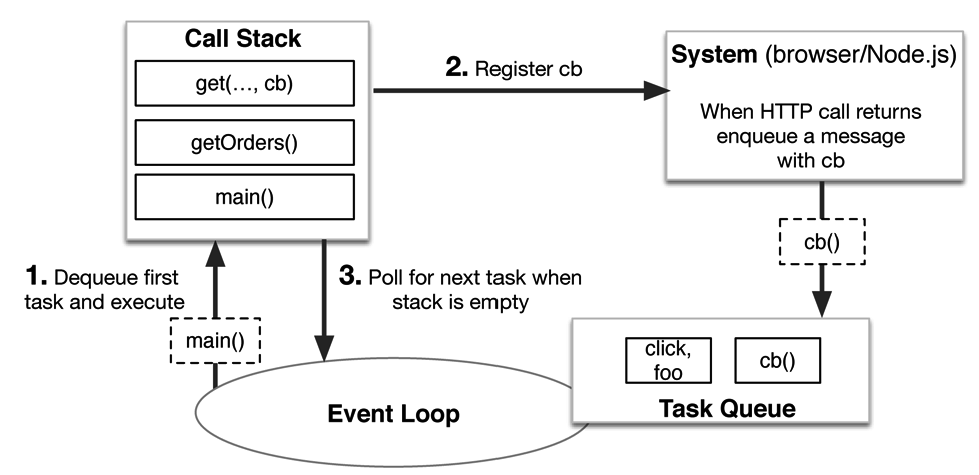
\includegraphics[width=\textwidth]{Images/Gallaba,Mesbahetal.png}
			\caption[Das JavaScript Event Loop Modell]{\label{JavaScriptEventLoop}Das JavaScript Event Loop Modell\\(aus \citep[S.~2]{Gallaba.b})}
		\end{figure}
		
		Der Ablauf der Nachrichtenverarbeitung und des Einreihens neuer Nachrichten durch die Laufzeitumgebung ist in Abbildung \ref{JavaScriptEventLoop} dargestellt. 
		
		Der Programmlauf startet mit der ersten Funktion der JavaScript Applikation (Schritt~1).  
		Während der Beispielausführung wird ein HTTP-Request über eine Bibliotheksfunktion der Laufzeitumgebung abgesetzt. Zusammen mit dieser Abfrage wird eine Callback-Funktion registriert (Schritt~2).  Sobald eine Antwort auf die Anfrage eintrifft, wird eine entsprechende Nachricht in die Queue eingereiht, die mit der Ausführung der Callback-Funktion assoziiert ist. 
		Wenn die Ausführung des aktuellen Codeabschnitts auf dem Stack beendet ist, tickt die Event-Loop und entnimmt die nächste Nachricht aus der Queue (Schritt~3).  Nach einer gewissen Anzahl Ticks wird so auch die vorher eingereihte Nachricht verarbeitet und die assoziierte Callback-Funktion wird ausgeführt.
		
	\subsection{Single Thread Modell und Run-to-Completion Semantik}
		Eine wichtige Eigenschaft von ECMAScript ist in diesem Ablauf die durch den Standard garantierte Beschränkung der Programmausführung auf einen einzigen Thread.\footnote{Die ECMAScript~6 Spezifikation dazu:
			\begin{quote}At any point in time, there is at most one execution context that is actually executing code. This is known as the running execution context.~\citep[\S~8.3]{EcmaTC39.}\end{quote} und
			\begin{quote}Execution of a Job can be initiated only when there is no running execution context and the execution context stack is empty.~\citep[\S~8.4]{EcmaTC39.}\end{quote}}
		Dadurch ist garantiert, dass eine einmal zur Ausführung gekommene Funktion nicht durch andere Funktionen unterbrochen werden kann. Jeder Eintrag in der Queue wird vollständig abgearbeitet, bevor die nächste Nachricht entnommen und verarbeitet werden kann.
		
		Dieses Verhalten ist unter dem Namen "`Run-To-Completion"'-Seman"-tik bekannt und unterscheidet JavaScript von multi-threaded Programmiersprachen wie z. B. Java, in denen die Programmiererin damit rechnen muss, dass ihr laufender Code zu jeder Zeit vom Code eines anderen Threads inner\-halb ihrer Applikation unterbrochen werden kann.
		
		\paragraph{Konsequenzen und Vorteile}
		
		Dass die Codeausführung nicht unterbrochen werden kann, erinnert an alte Zeiten von kooperativen Multitasking Systemen. Dort konnte ein einzelner lang laufender Prozess das System unbedienbar machen oder sogar zum Absturz bringen. Die Situation in JavaScript ist ähnlich: Eine einzelne lang laufende Operation kann die Ausführung anderer, eigentlich nebenläufiger, Prozesse verzögern oder sogar verhindern. Im Browser wird dann die Meldung "`Script takes too long to run"' angezeigt (vgl.~\citep{MozillaDeveloperNetwork.2016}). 
		
		Für die Javascript Programmiererin ist es unerlässlich durch geeignete Maßnahmen wie asynchrone Programmierung dafür zu sorgen, dass eine Funktionsausführung den Stack nicht zu lange blockiert. Dies wird nicht durch die Laufzeitumgebung sichergestellt, sondern liegt einzig in der Hand der Programmiererin. Sie ist dafür verantwortlich, dass die Event-Loop nicht blockiert wird. 
		
		In anderen Programmiersprachen ist es möglich und üblich für lang laufende Operationen einen eigenen Thread abzuspalten, der dann pa\-ral\-lel zur weiteren Programmausführung abläuft. Das Umschalten zwischen den Threads einer Anwendung wird durch das Laufzeitsystem bzw. das Betriebssystem übernommen und erfolgt präemptiv. Dadurch bekommen die Threads einen fairen Anteil an Rechenzeit oder können ganz suspendiert werden, wenn sie z. B. auf I/O-Operationen warten.
		
		Das Single-Thread Ausführungsmodell mit seiner Run-to-Completion Semantik scheint auf den ersten Blick nebenläufige Code-Ausführung zu verhindern und ein klarer Nachteil gegenüber multi-threaded Systemen zu sein. Nicht umsonst haben sich auf dem Desktop präemptive Multitasking-Betriebssysteme durchgesetzt, die auch dann noch bedienbar bleiben, wenn ein einzelner Prozess nicht mehr reagiert.
		
		Der Vorteil des Multi-Threading wird aber durch zwei neue Probleme erkauft: 
		
		Die Verwaltung und das Scheduling von Threads kosten erhebliche Resourcen. Dies wird von Ryan Dahl bei der Vorstellung des Node.js Konzepts anhand des multi-threaded Webservers Apache im Vergleich zum Event-Loop getriebenen single-threaded Server NGINX eindrücklich präsentiert (vgl.~\citep{Dahl.2009} ab $\sim$3:00 und den Blogpost~\citep{Poli.2013}).
		
		Das andere Problem in einer multi-thread Umgebung ist die Synchronisation. Jeder Programmteil muss jederzeit damit rechnen, dass die Ausführung unterbrochen wird und zwischenzeitlich anderer Code abläuft. Die Verantwortung dafür, dass die Daten und Objekte der Applikation trotzdem in einem konsistenten Zustand bleiben, liegt bei der Programmiererin. Oft muss erheblicher Aufwand zur Synchronisation getrieben werden. Solche Synchronisationsprobleme können in einer reinen single-thread Umgebung wie JavaScript gar nicht erst auftreten. Dave Herman schreibt dazu sehr treffend: 
		
		\begin{quote}Part of the beauty of JavaScript's event loop is that there's a very clear synchronization point for reaching a stable state in your programs: the end of the current turn. You can go ahead and leave things in a funky intermediate state for as long as you like, and as long as you stitch everything back up in time for the next spin of the event loop, no other code can run in the meantime. That means you can be sure that while your object is lying in pieces on the floor, nobody else can poke at it before you put it back together again.~\citep{Herman.01.04.2016}
		\end{quote}
		

\section{Asynchrone Programmierung}
		Wie können trotz der Beschränkung auf einen einzigen Thread performante Programme geschrieben werden, die die Event-Loop nicht blockieren und auch bei länger laufenden Operationen reaktiv und bedienbar bleiben? 
		
		Die allermeisten Anwendungen sind selber nicht sehr rechenintensiv, benutzen jedoch externe Funktionen, die vergleichsweise lange brauchen, um ein Ergebnis zu liefern. Typischerweise sind dies alle Arten von I/O-Ope"-ra"-ti"-onen, Netzwerkzugriffen und Datenbankabfragen. 
		In Tabelle \ref{tab:latencies} sind Latenzzeiten von beispielhaften Operationen angegeben. Diese werden zwar häufig durch eigenen Code ausgelöst bzw. aufgerufen, sie laufen jedoch nicht innerhalb der eigenen Applikation ab.
		Damit solche Aufrufe nicht die gesamte Anwendung blockieren, muss eine konkurrenzfähige Programmiersprache eine Form der Nebenläufigkeit (Concurrency) unterstützen.
			
		\begin{table}[h]\centering
			% Table generated by Excel2LaTeX from sheet 'Tabelle1'
			\begin{tabular}{l|r}
				\hline
				\textbf{Operation} & \textbf{Latency} \\
				\hline\hline
				L1 cache reference &     0.5 ns \\
				\hline
				Branch mispredict &       5 ns \\
				\hline
				L2 cache reference &       7 ns \\
				\hline
				Mutex lock/unlock &      25 ns \\
				\hline
				Main memory reference &     100 ns \\
				\hline
				Compress 1K bytes with Zippy &   3,000 ns \\
				\hline
				Send 2K bytes over 1 Gbps network &  20,000 ns \\
				\hline
				Read 1 MB sequentially from memory & 250,000 ns \\
				\hline
				Round trip within same datacenter & 500,000 ns \\
				\hline
				Disk seek & 10,000,000 ns \\
				\hline
				Read 1 MB sequentially from disk & 20,000,000 ns \\
				\hline
				Send packet CA->Netherlands->CA & 150,000,000 ns \\
				\hline
			\end{tabular}  
			\caption[Vergleich unterschiedlicher Latenzen typischer Operationen]{Vergleich unterschiedlicher Latenzen typischer Operationen. \protect\\(Daten aus~\citep[S.~13]{Dean.2007})}
			\label{tab:latencies}
		\end{table}
		
		Die JavaScript Event-Loop unterstützt genau solch eine Nebenläufigkeit, wenn es zwar lang dauert bis ein Ergebnis vorliegt, diese Latenz aber nicht durch große Rechenlast verursacht wird, sondern durch das Warten auf externe Operationen, die außerhalb der eigenen Applikation ablaufen. 
	

	\subsection{Non-Blocking Function Calls}
	In traditionellen Programmiersprachen ist man es gewohnt, dass ein Funktionsaufruf mittels eines \textsf{return} ein Ergebnis zurückgibt. Diese Ergebnisrückgabe an die aufrufende Funktion erfolgt, wenn das Ergebnis auch wirklich vorliegt. Der aufrufende Code ist solange blockiert bis er die Ablaufkontrolle zusammen mit dem Ergebnis explizit per \textsf{return} zurück bekommt.
	
	Eine solche Art der Programmausführung führt in einer single-thread"-ed Sprache zu sehr ineffizienten Programmen, da während der Wartezeit keine anderen Aktionen ausgeführt werden können. 
	
	Um diese Situation aufzulösen, muss es möglich sein die Rückgabe der Ablaufkontrolle mittels \textsf{return} und die Bereitstellung des Ergebnisses einer Funktion voneinander zu entkoppeln. Das Anstoßen einer externen Operation darf den Programmablauf nicht blockieren.
	
	Dieses Verhalten zeigen nicht-block"-ierende Funktionsaufrufe (non-blocking function calls). Sie stoßen eine externe Aktion lediglich an und kehren sofort zurück, bevor das angeforderte Ergebnis vorliegt. Das Programm kann währenddessen mit anderen Aufgaben fortfahren und wird informiert, wenn das Ergebnis verfügbar ist. Die angestoßene Aktion läuft dabei in der Regel außerhalb des eigenen Single-Threads ab.\footnote{vgl. dazu:
		\begin{quote}[...]the JavaScript code you write all runs on a single thread, but the code that implements the async task ([...]) is not part of that JavaScript and is free to run in a separate thread.~\citep[S.~7]{Parker.2015}\end{quote}}
	
	\subsection{\emph{Jetzt} und \emph{Später}}
	
	Die Applikation kann eine Aktion \emph{jetzt} anstoßen, wird dadurch aber nicht blockiert, sondern kann direkt weiterlaufen. Das Ergebnis liegt erst zu einem noch unbekannten Zeitpunkt in der Zukunft vor und wird \textit{später} verarbeitet. 
		
	Ein solches Programmiermodell wird als "`asynchrone Programmierung"' bezeichnet.
	Deren Kern besteht in der Entkopplung zwischen der \textit{jetzt} statt"-fin"-den"-den Auslösung einer Aktion und dem \textit{späteren} Vorliegen und Verarbeiten eines Ergebnisses.
	
	\begin{quote}In fact, the relationship between the \textit{now }and \textit{later }parts of your program is at the heart of asynchronous programming.~\citep{Simpson.2015}\end{quote}
	
	Im Gegensatz zur synchronen Programmierung kann man sich in der asynchronen Programmierung den Programmablauf nicht mehr als linearen Zeitstrahl vorstellen, bei dem jede Ursache (ein Funktionsaufruf) direkt eine Wirkung (die Rückgabe des Ergebnisses) nach sich zieht. Vielmehr wird die Programmabarbeitung in kleinere Einheiten unterteilt, welche zwar kausal voneinander abhängen, deren zeitlicher Ablauf jedoch voneinander entkoppelt ist. Ein Programm kann daher immer weiter laufen, ohne dass es blockierend auf Ergebnisse einer von ihm angestoßenen Aktion warten muss.
	
	Die \textit{spätere} Verarbeitung des Ergebnisses ist garantiert. Es ist jedoch unbekannt, wann genau das Ergebnis tatsächlich verarbeitet wird.\footnote{vgl. dazu: \begin{quote}After the callback is added to the queue, there is no guarantee how long it will have to wait. How long it takes the current code to run to completion and what else is in the queue controls the time. The queue can contain things such as mouse clicks, keystrokes, and callbacks for other async tasks.~\citep[S.~7]{Parker.2015}\end{quote}}
	
	Durch die konsequente Nutzung asynchroner Programmierung mit non-blocking function calls ist es möglich Programme zu schreiben, die durch den Verzicht auf internes Multi-Threading sehr performant und mit hohem Durchsatz ausgeführt werden können. Während externe Ergebnisse bereitgestellt werden kann die Applikation weiterlaufen (vgl.~\citep{Dahl.2009}). 
	
	
	\subsection{Asynchrone Programmierung in JavaScript}
	
	Die Entkopplung zwischen \emph{jetzt} und \emph{später} wird in JavaScript über die Event-Loop des Laufzeitsystems erreicht. \emph{Jetzt} bezeichnet den aktuellen Tick der Event-Loop, bis der Stack wieder geleert ist. Alle Code\-ab\-schnitte, die mit einem weiteren Ereignis der Queue assoziiert sind, werden \emph{später} ausgeführt.
	
	Der Code in jedem Tick der Event-Loop läuft dabei wie gewohnt sequentiell ab. Die Ergebnisse von non-blocking function calls werden als Ereignisse in die Queue einsortiert und damit \emph{später} verarbeitet. 
	
	In der JavaScript Praxis ist das Konzept der asynchronen Programmierung so erfolgreich, dass z. B. Node.js (fast) vollständig auf non-blocking function calls setzt\footnote{Ryan Dahl dazu in einem Interview:~\begin{quote}Everything is a callback. So where you would traditionally say: "`access the database, write to file, move file over there and do something else"' you kind of do these sequential sort of actions one after another. In Node you can't do those sort of things because you might take some amount of time for you to move a file from one place to another because the disk might have to spin, or if you query your database that might take some milliseconds for you to respond and in Node everything is non-blocking and so it doesn't allow you to just sit there and then return the response.~\citep{Dahl.2010}\end{quote}}
	und auch im Bereich der Web"-applikationen im Browser die Zahl der asynchron arbeitenden Application Programming Interfaces (API) rapide zunimmt.\footnote{vgl. dazu: \begin{quote}The number of asynchronous JavaScript APIs is rapidly growing.~\citep[S.~1]{Parker.2015}\end{quote}}


\section{Callbacks in traditionellem \-JavaScript}

	Um die eben erläuterte asynchrone Programmierung in JavaScript zu realisieren, ist ein Mechanismus notwendig, die \emph{später} vorhandenen Ergebnisse in den Programmablauf einzuspeisen und weiter zu verarbeiten. In traditionellem JavaScript wird dazu der aufgerufenen asynchronen Funktion eine sogenannte "`Callback-Funktion"' als Parameterargument übergeben. Diese kann ausgeführt werden, sobald das Ergebnis des asynchronen Aufrufs vorliegt, und dieses verarbeiten. 
	
	\begin{quote}The callback function is the async work horse for JavaScript, and it does its job respectably.~\citep[S.~26]{Simpson.2015}\end{quote}

	
	\subsection{Funktionsweise von Callbacks}

	Die Callback-Funktion wird beim asynchronen Aufruf übergeben und soll \emph{später} das Ergebnis verarbeiten. 
	Das eigene Programm läuft nach der sofortigen Rückkehr aus dem nicht-blockierenden Funktionsaufruf \textit{jetzt} weiter. 	
	Die asynchrone Funktion dagegen wird außerhalb des aktuellen Execution-Context des Hauptprogramms ausgeführt und ermittelt letztendlich ein Ergebnis (Erfolg oder Fehler). Um dieses Ergebnis an das Hauptprogramm zurückzuliefern, wird der Aufruf der Callback-Funktion als Nachricht in die Queue der Laufzeitumgebung eingestellt. Das Ergebnis selber wird der Callback-Funktion als Aufrufparameter übergeben. Die Event-Loop bringt die übergebene Callback-Funktion zu einem \emph{späteren} Zeitpunkt zur Ausführung, so dass sie das Ergebnis im Rahmen des Hauptprogramms verarbeiten kann.\footnote{	
	Eine interessante Sichtweise dieses Prozederes besteht darin die übergebene Callback-Funktion als "`Continuation"' aufzufassen: Die aufrufende Funktion übergibt der aufgerufenen den "`nächsten Schritt"' des Hauptprogramms (eine Continuation) zur Verarbeitung des Ergebnisses. Diese Sichtweise und Art der Programmierung wird auch als "Continuation Passing Sytle" (CPS) bezeichnet. (vgl.~\citep{Rauschmayer.2012})}

	Ein Beispiel für einen asynchronen Aufruf mit Ergebnisübergabe per Callback ist in Listing \ref{snippets/callbackErrorFirstEx.js} zu sehen. Der vierte Parameter für \textsf{asyncCall} ist die Callback-Funktion, die an Ort und Stelle als anonyme Funktion inline definiert wird.
	
	\insertcode{snippets/callbackErrorFirstEx.js}{Beispiel für einen asynchronen Aufruf mit Callback.}
	
	\paragraph{Konventionen} 
	Prinzipiell sind als Schnittstelle zwischen eigenem Programm, asynchronen Aufrufen und Callbacks beliebige Funktionen mit beliebigen Signaturen zulässig. 
	In der Javascript Praxis haben sich aber Konventionen herausgebildet, die eine gewisse Durchgängigkeit bringen und den Wildwuchs von Schnittstellen eindämmen.
	Am Beispiel in Listing \ref{snippets/callbackErrorFirstEx.js} lassen sich die Konventionen "`trailing callback"' und "`error first"' erläutern.

	\paragraph{Trailing Callback} In den meisten Funktionen, die einen Callback akzeptieren, wird dieser als letzter Parameter in der Funktions-Signatur angegeben. Diese Konvention wird als "`trailing callback"' bezeichnet und ist insbesondere bei Modulen für die Node.js Laufzeitumgebung häufig anzutreffen. 
	
	Diese letzte Parameter-Position für den Callback verbessert die Lesbarkeit erheblich, wenn als Callback-Funktion anonyme Funktionen verwendet werden, die sich über mehrere Zeilen erstrecken.  
	
	Auch existieren mittlerweile viele APIs, bei denen die Angabe einer Call"-back-Funktion optional ist. 
	In diesem Fall ist es notwendig, dass die aufgerufene Funktion überprüfen kann, ob ihr eine Funktion als Callback-Parameter übergeben wurde oder nicht. Dies wird wesentlich erleichtert, wenn der optionale Callback-Parameter an einer ausgezeichneten (der letzten) Position in der Parameterliste steht.
	
	\paragraph{Error First} 
	In sehr vielen APIs hat sich das sogenannte "`error-first"' Protokoll für Callbacks durchgesetzt. Diese Konvention besagt, dass eine Callback-Funktion die festgelegte Signatur \textsf{cb(err,~result)} besitzt.
	In der Callback-Funktion selber wird geprüft, ob der \textsf{err}-Parameter angegeben wurde. Wenn dieser vorhanden ist, dann wird eine Fehlerbehandlung durchgeführt. Wenn dieser erste \textsf{err}-Parameter nicht gesetzt ist, dann wird das im folgenden \textsf{result}-Parameter übergebene Ergebnis verwendet und verarbeitet.\footnote{Die Firma Joyent, welche die initiale Entwicklung von Node.js gesponsort hat, dazu in ihren Best Practices:\begin{quote}The usual pattern is that the callback is invoked as callback(err, result), where only one of err and result is non-null, depending on whether the operation succeeded or failed.~\citep{Joyent.}\end{quote}}
	

	\subsection{Problematik traditioneller Callbacks}
	Die Übergabe einer Callback-Funktion an die aufgerufene asynchrone Funktion, welche diese dann ihrerseits mit ihrem Ergebnis aufruft, stellt die traditionelle Methode zur asynchronen Programmierung in Java"-Script dar. In den JavaScript Versionen vor ECMAScript~6 gab es keine andere Methode asynchrone Programmierung zu realisieren.
	
	Doch ist dieses Vorgehen nicht frei von Problemen, welche im Folgenden aufgezeigt werden sollen.
	
	\subsubsection["`Pyramid of Doom"']{"`Pyramid of Doom"' und schlechte Nachvollziehbarkeit}
	
	Häufig sind mehrere asynchrone Funktionen voneinander abhängig. Im Beispiel Listing \ref{snippets/nestedCallbacks.js} wird zunächst eine Datenbankverbindung aufgebaut. Sobald diese Verbindung aufgebaut ist, wird eine Anfrage an die Datenbank abgesendet. Schließlich wird das angefragte Datum an den zu Beginn übergebenen Callback übergeben und dort verarbeitet.
	
	\insertcode{snippets/nestedCallbacks.js}{Beispiel zu "`nested Callbacks"' bei voneinander abhängigen asynchronen Funktionsaufrufen}
	
	Abhängige asynchrone Aufrufe führen zu verschachtelten Callbacks, deren Code durch die immer weiter voran schreitende Einrückung schnell schwer lesbar und unübersichtlich wird.
	 Diese immer weiter voran schreitende Einrückung im Quelltext ist unter dem treffenden Namen "`Pyramid of Doom"' hinlänglich bekannt. (vgl.~\citep[\S~1]{KennedyKambona.2013})
	
	Bei solchen verschachtelten Callbacks ist jedoch nicht in erster Linie die Formatierung des Quelltexts problematisch. Vielmehr ist es für die Programmiererin schwierig nachzuvollziehen, welche Ausführungspfade tatsächlich eingeschlagen werden und welche zeitliche Abfolge sich ergibt.\footnote{Das menschliche Gehirn ist auf die Verarbeitung von linearen Prozessen ausgelegt, die nacheinander ablaufen. (vgl. "`Sequential Brain"' in~\citep[~27ff.]{Simpson.2015}) Durch die Benutzung von asynchronem Code mit Callbacks wird dieser normale Denkablauf stark gestört und es fällt Menschen schwer, die genauen Abläufe mit all ihren zeitlichen und datengetriebenen Abhängigkeiten nachzuvollziehen und zu planen. Siehe dazu \citep{KennedyKambona.2013}: 
		
		\begin{quote}Since callbacks are common in JavaScript, programmers end up losing the ability to think in the familiar sequential algorithms and end up dealing with an unfamiliar program structure.\end{quote}} Insbesondere in Zusammenhang mit der Fehlerbehandlung ergeben sich in der Praxis sehr schnell äußerst unübersichtliche Strukturen.\footnote{In realem Code kommen überwiegend zwei bis drei Schachtelungsebenen vor. Jedoch gibt es Beispiele von bis zu 8 Eben tiefen Callback-Schachtelungen. (vgl. dazu~\citep[\S~IV.D]{Gallaba.b})}

	\subsubsection{Komplizierte Fehlerbehandlung} 
	In synchronem JavaScript Code wird das Error-Handling über einen \textsf{try-catch-finally}-Mechanismus behandelt. Wenn in einer Funktion ein nicht behebbarer Fehler auftritt, so wird mittels \textsf{throw} die Funktion vorzeitig mit einem Fehlerobjekt verlassen. In einer weiter außen liegenden Programmschicht -- also in einem auf dem Stack weiter unten liegenden Execution-Context -- kann dieser Fehler mittels einer \textsf{catch}-Klausel abgefangen und behandelt werden. Die Installation eines generischen Error-Handlers, der in einem bestimmten Applikations-Kontext alle bis dahin unbehandelten Fehler fängt und behandelt, ist im synchronen Fall über den \textsf{try-catch-finally}-Mechanismus relativ leicht möglich. 
	
	Im Fall der asynchronen Programmierung versagt dieser Sprachmechanismus. Der asynchrone Code läuft in einem anderen Ausführungskontext ab als die aufrufende Funktion. Es ist keine weiter außen liegende Programmschicht vorhanden, welche den Fehler im Kontext des Funktionsaufrufs der asynchronen Funktion behandeln könnte. Ein mit \textsf{throw} geworfener Fehler müsste von einem Error-Handler verarbeitet werden, der keine Kenntnis davon hat, aus welchem Kontext heraus der vorliegende Fehler entstanden ist.\footnote{vgl. dazu: \begin{quote}In synchronous JavaScript code the throw keyword can be used to signal an error and try/catch can be used to handle the error. When there is asynchrony, however, it may not be possible to handle an error in the context it is thrown. Instead, the error must be propagated asynchronously to an error handler in a different context.~\citep[S.~2]{Gallaba.b}\end{quote}}
	
	Um einen extern zur Applikation auftretenden Fehler im Applikationskontext behandeln zu können, muss der Fehler genau wie ein Ergebnis wieder zurück in einen anderen Kontext übergeben werden. 	Dazu dient z. B. das erwähnte Error-First-Protokoll (vgl. Listing~\ref{snippets/callbackErrorFirstEx.js}). Die Fehlerbehandlung muss aber für jeden einzelnen asynchronen Aufruf explizit ausprogrammiert werden, wobei viele verschiedene Ausführungspfade berücksichtigt werden müssen. Dazu muss eine große Menge "`Boiler"-plate-Code"' geschrieben werden, der sowohl unübersichtlich als auch schlecht wiederverwendbar ist. Die Gefahr ist groß, dass bestimmte Fehlerfälle bei dieser expliziten Behandlung vergessen werden und im besten Fall "`silently swallowed"' werden, also unbehandelt bleiben und im schlechtesten Fall die Applikation zum Absturz bringen.
	
	\subsubsection{Inversion of Control}
	Ein weiteres Problem bei der Übergabe von Callbacks an die asynchrone Funktion ist die Umkehrung der Ausführungskontrolle ("`Inversion of control"'). Durch die Übergabe eines Callbacks wird die Kontrolle über den weiteren Programmablauf vom Hauptprogramm an die aufgerufene Funktion abgegeben. Die aufgerufene Funktion ist für die Ausführung der übergebenen Callback-Funktion (der Continuation) verantwortlich. Das ist eine Inversion of Control, in der das aufrufende Programm keinen Einfluss mehr darauf hat, in welcher Art und Weise der an die aufgerufene Funktion übergebene "`nächste Schritt"' ausgeführt wird.
	
	Häufig handelt es sich bei den aufgerufenen Funktionen um fremden Code (3$^\mathrm{rd}$ Party Code, externe Bibliotheken, \ldots), der nicht als Quelltext zur Überprüfung vorliegt oder so komplex ist, dass eine Überprüfung aus praktischen Gründen ausscheidet.
	Die Programmiererin ist also darauf angewiesen der aufgerufenen Funktion zu vertrauen, dass diese den übergebenen Callback korrekt aufruft. Sie gibt damit die Kontrolle über den weiteren Ablauf des Programms aus der Hand.
	
	Natürlich ist beim Aufruf externer Funktionen immer ein gewisses Maß an Vertrauen darauf notwendig, dass die fremde Funktion so funktioniert wie versprochen und ein korrektes Ergebnis gemäß ihrer Spezifikation liefert. Während in synchronem Code jedoch der schlimmste eintretende Fall darin besteht, dass ein inkorrektes Ergebnis zurückgegeben wird oder eine Ausnahme ausgelöst wird, so hat ein falsch verwendeter Callback direkte Auswirkungen auf den weiteren Ablauf des eigenen Programms. Der fremde Code könnte (vgl.~\citep[S.~48]{Simpson.2015})
	\begin{itemize}[nosep]
		\item den Callback zu früh, also synchron anstatt asynchron, aufrufen,
		\item den Callback zu spät oder gar nie aufrufen,
		\item den Callback zu selten oder zu oft aufrufen,
		\item auftretende Fehler oder Ausnahmen verschlucken.
	\end{itemize}

	Insbesondere der erste Punkt stellt ein subtiles Problem bei der Übergabe von Callbacks an Fremdcode dar. Es ist einer aufgerufenen Funktion nicht anzusehen, ob sie intern wirklich asynchron arbeitet, den Callback also \textit{später} ausführt oder ob es bestimmte Situationen gibt, in denen der Callback vielleicht doch synchron ausgeführt wird. Durch ein solches Verhalten wird eine Verzweigung im Ausführungspfad des Programms eingeführt, die den Code deutlich komplexer macht. Insbesondere wird die Run-to-Completion Semantik gebrochen, bei der die Programmiererin sich darauf verlassen kann, dass der eigene \-\-Code vollständig abgearbeitet wird, bevor die Callback-Funktion aus dem asynchronen Aufruf heraus ausgeführt wird.\footnote
	{
		Das Verhalten, dass eine Callback Funktion in manchen Fällen synchron und in anderen asynchron ausgeführt wird, ist in der Javascript-Community inzwischen weithin als "`Release of ZALGO"' bekannt und sollte unbedingt vermieden werden. Die Bezeichnung für das Phänomen geht auf den inzwischen berühmten Blogpost von Isaac Schlüter zurück ~\citep{Schlueter.2013}. 
		
		Um eine Vermischung von synchroner und asynchroner Ausführung zumindest im eigenen \-Code zu vermeiden, sollte man den folgenden Rat beherzigen: 
		
		\begin{quote}
			You can see just how quickly the unpredictability of Zalgo can threaten any JavaScript program. So the silly-sounding "`never release Zalgo"' is actually incredibly common and solid advice. Always be asyncing.~\citep[S.~37]{Simpson.2015}
		\end{quote}
		Das bedeutet, dass man den Aufruf eines übergebenen Callbacks immer zur \emph{späteren} Ausführung in de Queue einreihen sollte, selbst wenn das Ergebnis im speziellen Fall schon \emph{jetzt} zur Verfügung steht.
		
		Eine bekannte Funktion, die gegen diesen Rat verstößt und ihren Callback je nach Situation synchron oder asynchron ausführt, ist z. B. die Funktion \textsf{jQuery.ready(cb)}.
	}

	Obwohl Gefahren bei den anderen genannten Punkten offensichtlicher sind, und damit leichter auffallen, stellen auch sie eine erhebliche Fehlerquelle für die korrekte Programmausführung dar. 
	
	Bei der Übergabe einer Continuation in Form eines Callbacks an eine asynchrone Funktion muss die Programmiererin darauf vertrauen, dass diese korrekt arbeitet. Selbst die ausführlichsten Tests können allenfalls Indizien liefern, die dieses Vertrauen rechtfertigen. 
	
	\subsection{Bewertung traditioneller Callbacks}
		Die vorigen Abschnitte haben deutlich gezeigt, dass die Übergabe von Callbacks zur Verarbeitung asynchroner Ergebnisse zwar einfach zu realisieren ist, aber im Detail einige Probleme bereit hält. Diese reichen von Verständnisproblemen, die eher lästig sind, über eine aufwändige Fehlerbehandlung bis hin zu schwerwiegenden Vertrauensproblemen im Zusammenhang mit dem \-Code von Dritten.
		
		Obwohl der Callback-Mechanismus das Fundament der asynchronen Programmierung darstellt, führen die angesprochenen Probleme zu der in der JavaScript Community weithin bekannten "`Callback Hell"'.
		
		\begin{quote}
			\textbf{That }is what "`callback hell"' is all about! The nesting/indentation are basically a side show, a red herring.~\citep[S.~32]{Simpson.2015}
		\end{quote}

\section{Moderne Methoden in ECMAScript 6}
	Wie jede lebendige Programmiersprache entwickelt sich auch Java\-Script beständig weiter. Es werden laufend neue Konzepte entwickelt, um die Verwendung der Sprache zu erleichtern und sicherer zu machen. In JavaScript werden solche neuen Konzepte häufig zunächst mit den Mitteln des aktuell gültigen Sprachstandards entwickelt und über sogenannte Polyfills\footnote{
	Als Polyfill bezeichnet man ein Stück JavaScript \-Code, der neuere Sprach\-fea\-tures per Bibliotheksfunktion auch in älteren Laufzeitumgebungen verfügbar macht. Diese Technik wird oft benutzt, um z.~B. in Webbrowsern die unterschiedliche Unterstützung neuerer Funktionen auszugleichen. Je nach verwendetem Browser wird ein passender "`Polyfill"' mit der Webseite ausgeliefert, so dass die Programmiererin für alle Plattformen die gleichen Funktionen und APIs nutzen kann. (vgl.~\citep{Sharp.2010})}
	implementiert. Wenn sich die neu entwickelten Sprachmittel in der Praxis bewähren, können sie in den Sprachstandard aufgenommen werden.\footnote{Zur Aufnahme neuer Features in den Sprachstandard vgl. den Prozess in \citep{EcmaTC39committee.2016}.}

	\paragraph{Neue Sprachmittel: Promises und Generators}
	In der Javascript Community wurden auch Konzepte entwickelt, um die asynchrone Programmierung zu erleichtern und der Callback-Hell zu entkommen. Insbesondere "`Promises"' und "`Generators"' sind dazu geeignet, die im vorigen Abschnitt angesprochenen Probleme traditioneller Callbacks zu lösen. Diese beiden Konzepte fanden Aufnahme in den ECMAScript~6 Standard (vgl.~\citep{EcmaTC39.}) und sind seitdem Teil aller kompatiblen Sprachimplementierungen.
		
	Die Konzepte "`Promises"' und "`Generators"' sollen in diesem Kapitel als moderne Antwort auf die traditionellen Callbacks in JavaScript detailliert erläutert werden.

	\subsection{Promises}
	
	Wenn die Übergabe von Callbacks an asynchrone Funktionen zur \emph{späteren} Verarbeitung der Ergebnisse offensichtlich problematisch ist, so stellt sich zwangsläufig die Frage nach Alternativen:
	
	\begin{quote}What if instead of handing the continuation of our program to another party, we could expect it to return us a capability to know when its task finishes, and then our code could decide what to do next?~\citep[S.~39]{Simpson.2015}\end{quote}
	
		\subsubsection{Die Idee von Promises}
			Interessanterweise ist schon lange ein Konzept bekannt, welches genau das leistet: Promises als Platzhalterobjekt für Ergebnisse, die erst in \textit{späterer} Zukunft vorliegen.
			
			Anstatt der asynchron aufgerufenen Funktion die Continuation ihres Programms anzuvertrauen, erhält die Programmiererin ein Platzhalterobjekt zurück, das letztendlich nach Abschluss der asynchronen Operation deren Ergebnis enthält.
			
			Dieses Konzept wurde 1976 in einem Paper ~\citep[S.~263]{Friedman.1976} das erste Mal für die Parallelisierung von funktionaler "`Lazy Evaluation"' in Mehrprozessorsystemen vorgestellt und dort als "`Promise"' benannt: 
			
			\begin{quote}in fact [\ldots] z is initially bound only to a "`promise"' of this result.~\citep[S.~268]{Friedman.1976}\end{quote} 
			
			Obwohl das dort vorgestellte Konzept einen anderen Ausgangspunkt hatte, waren die damit gelösten Probleme doch denen der asynchronen Programmierung sehr ähnlich:
			
			\begin{quote}
				The colonel behaves exactly as a single processor would, except that from time to time it accesses what would have been a suspension and instead finds the result already provided by a sergeant who had passed through earlier.~\citep[S.~269]{Friedman.1976}
			\end{quote} 
			Der sogenannte "`Colonel"' Prozess läuft auf einem einzigen Thread und bekommt von parallel in anderen Ausführungskontexten arbeitenden "`Sergeants"' Ergebnisse geliefert, mit denen er weiterarbeiten kann.
			
			Die erste bekannte Implementierung von Promises, um explizit asynchrone Prozeduraufrufe aufzulösen, wurde 1988 in~\citep[S.~260]{Liskov.1988} vorgestellt. Die dort vorgestellten Promises geben schon 27 Jahre bevor die eingangs dieses Abschnitts zitierte Frage gestellt wurde eine zufriedenstellende Antwort darauf: 
			
			\begin{quote}Promises allow a caller to run in parallel with a call and to pick up the results of the call, including any exceptions it raises, in a convenient and type-safe manner.~\citep[S.~260]{Liskov.1988}\end{quote}
			
			\paragraph{Geänderte Aufrufsemantik von asynchronen Funktionen} Beim bisherigen Konzept zum Aufruf asynchroner Funktion wurde diesen eine Callback-Funktion übergeben, welche nach Beendigung der asynchronen Aufgabe zur Rückgabe des Ergebnisses aufgerufen wurde. Bei der Verwendung von Promises wird die Situation umgedreht und die aufgerufene Funktion gibt direkt und synchron (also \textit{jetzt}) ein Promise-Objekt als Platzhalter für das zu einem \textit{späteren} Zeitpunkt vorliegende Ergebnis zurück. Diese Promise kann von der eigenen Applikation wie ein normales Objekt verwendet werden. Sie kann z. B. in einer Variable zwischengespeichert oder an eine andere Funktion weitergereicht werden. Wenn das Ergebnis des asynchronen Aufrufs in der Promise schließlich vorliegt, kann dieses weiterverarbeitet werden, ohne dass dazu vorher eine Continuation an die asynchrone Funktion herausgegeben werden müsste.
		
		\subsubsection{Promises nach dem Promise/A+ Standard}

			Das Konzept der Promises als Platzhalterobjekt für das Ergebnis einer asynchronen Operation ist auch in der Java"-Script Community schon seit längerem bekannt und es gibt eine ganze Reihe von Bibliotheken mit denen es umgesetzt werden kann. Um eine Interoperabilität dieses Konzepts zu erreichen, wurde der "`Promise/A+"'-Standard (vgl.~\citep{PromisesA+}) entwickelt, der eine Semantik für Promises definiert, an den sich die allermeisten Promise-Bibliotheken halten.\footnote{Eine populäre Ausnahme bildet die \textsf{jQuery}-Bibliothek, die erst ab Version 3.0 (9. Juni 2016) kompatibel zum Promise/A+ Standard ist. Die folgenden Ausführungen sind daher nicht auf ältere Versionen von \textsf{jQuery} anwendbar.} 
			
			Mit der Version 6 der ECMAScript Spezifikation finden Promises nach dem Promise/A+-Standard im Jahr 2015 auch Eingang in den JavaScript Sprachstandard und sind seitdem Teil aller kompatiblen Sprach"-im"-ple"-mentierungen (vgl.~\citep{EcmaTC39.}). Die Funktionsweise dieser Promises soll im folgenden detailliert erläutert werden.

			
			\skippingparagraph
			Eine Promise hat einen Wert und einen Status. Je nach Status ist der Wert der Promise schon bekannt, oder er wird erst später zugewiesen wobei der Status sich ändert.
			
			\paragraph{Status einer Promise}
			Einem Promise Objekt ist einer von drei Status zugeordnet:
			\begin{quote}Any Promise object is in one of three mutually exclusive states: \emph{fulfilled}, \emph{rejected}, and \emph{pending}:  
				\begin{itemize}[nosep]
					\item A promise \textsf{p }is fulfilled if \textsf{p.then(f, r) }will immediately enqueue a Job to call the function \textsf{f}.
					\item A promise \textsf{p }is rejected if \textsf{p.then(f, r) }will immediately enqueue a Job to call the function \textsf{r}.
					\item A promise is pending if it is neither fulfilled nor rejected.
				\end{itemize}
				A promise is said to be \emph{settled} if it is not pending, i.e. if it is either fulfilled or rejected.~\citep[\S~25.4]{EcmaTC39.}\end{quote}
			Diese drei Zustände einer Promise sind in Abbildung \ref{promiseStates} dargestellt.
			\begin{figure}[h]
				\center
				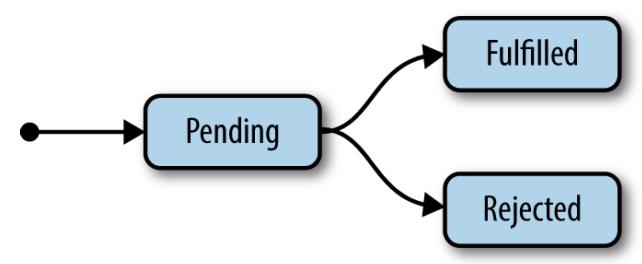
\includegraphics[width=0.5\textwidth]{Images/Parker2015-JavaScript.jpg}
				\caption[Die drei Status einer Promise]{\label{promiseStates}Die drei Status einer Promise.~(aus \citep[S.~16]{Parker.2015})}
			\end{figure}
			
			Solange in der asynchronen Funktion aus der die Promise zurückgegeben wurde noch kein Wert vorliegt, bleibt die Promise im Status \emph{pending}. Sobald die asynchrone Funktion ein Ergebnis ermittelt hat, wird dieses dem Wert der Promise zugewiesen und die Promise \emph{settled} damit. Ihr Status ändert sich entweder in \emph{fulfilled} oder \emph{rejected}. 
			
			Die Zuweisung an das Wertobjekt der Promise kann entweder ein Ergebniswert ("`value"'), ein Fehlerobjekt ("`reason"') oder aber eine weitere Promise sein. Der Normalfall ist die Zuweisung eines Ergebnisses mit dem Übergang in den Status \emph{fulfilled}. Falls bei der Ausführung der asynchronen Funktion ein Fehler auftritt, so bricht diese mit einem Fehlerobjekt ab und die Promise geht in den Status \emph{rejected} über. In beiden Fällen gilt die Promise als \textit{settled} und wird zu einem unveränderlichen (immutable) Objekt. 
			
			Wenn während des Settlements einer Promise diese als Wert eine weitere Promise zugewiesen bekommt, so übernimmt die äußere Promise Status und Wert der neu zugewiesenen inneren. Man spricht von "`lock-in"'. Verschachtelte Promises werden rekursiv aufgelöst, bis am Ende ein einzelnes Promise Objekt übrig bleibt welches entweder den Status \emph{fulfilled} oder \emph{rejected} annimmt.
			
			
			Diese Zustandsübergänge sind noch einmal in Abbildung \ref{promiseSettlement} angegeben.
			
			\begin{figure}[h]
				\centering
				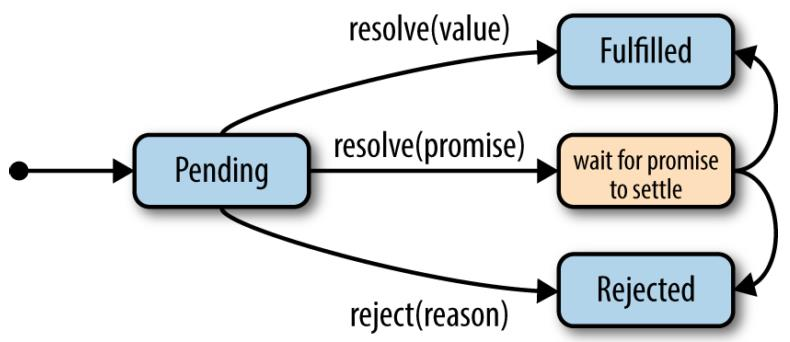
\includegraphics[width=0.5\textwidth]{Images/Parker2015-JavaScript(2).jpg}
				\caption[Settlement einer Promise]{\label{promiseSettlement}Settlement einer Promise mit verschiedenen Werten. (aus \citep[S.~17]{Parker.2015})}
			\end{figure}
			
			
			\paragraph{Signalisierung und Benutzung des Werts}
			Man kann einer Promise von außen nicht ansehen, in welchem Status sie sich gerade befindet. Der Status kann sich jederzeit von \emph{pending} zu \emph{settled} ändern. Um den endgültigen Wert einer erhaltenen Promise im eigenen \-Code zu verwenden, stellt jede Promise eine Methode \textsf{p.then(f, r)} bereit, die Handler-Funktionen registriert, welche ausgeführt werden, wenn eine Promise im Status \emph{settled} ist.
			Sie hat die Signatur \textsf{promise.then([f(val)], [r(val)]) returns promise}. 
			
			Jede Handler-Funktion \textsf{f(val)} und \textsf{r(val)} nimmt je einen Parameter. In diesem Parameter wird ihr der Wert der zugrundeliegenden (\emph{settled}) Promise übergeben. Dieser Wert kann dann verarbeiten werden. Die beiden Funktionsparameter \textsf{f} und \textsf{r} von \textsf{then([f], [r])} sind optional.
			
			Der Aufruf \textsf{p.then(f, r)} auf einer Promise \textsf{p} registriert die übergebenen Funktionen als Ergebnis-Handler für diese Promise. Der Handler \textsf{f} wird für die Verarbeitung des Wertes der Promise im Status \emph{fulfilled} registriert, der Handler \textsf{r} für die Verarbeitung des Wertes der Promise im Status \emph{rejected}. 
				
			Der Aufruf \textsf{p.then(f, r)} kann beliebig oft und zu beliebigen Zeiten auf einer Promise erfolgen. Bei mehrfachem Aufruf werden weitere Handler-Funktionen registriert. Die Promise selber wird immutable, sobald sie \emph{settled} ist und verändert sich durch weitere Registrierung von Handler-Funktionen nicht mehr.
			
			Wenn die Promise \emph{settled} ist, werden je nach Status entweder alle registrierten Fulfillment-Handler oder aber alle registrierten Rejection-Handler zur Ausführung gebracht. Wenn beim Aufruf von \textsf{p.then()} ein Parameter weggelassen wird und somit kein Handler für \emph{fulfilled} oder \emph{rejected} registriert wird, so wird der leere Standard-Handler ausgeführt. Da es relativ häufig vorkommt, dass nur der Rejection-Handler registriert werden soll, wurde in ES6 die Abkürzung \textsf{p.catch(r)} für den Aufruf \textsf{p.then(null, r)} eingeführt.
			
			Wird eine Handler-Funktion auf einer Promise registriert, die schon \emph{settled} ist, so wird die Ausführung des passenden Handlers direkt in die Queue eingereiht. Der Aufruf einer jeden Handler-Funktion erfolgt immer asynchron durch Einreihung in die Queue. Ein synchroner Aufruf des Handlers ist ausgeschlossen!
			
			
			\paragraph{Promise Chaining} 
			Die Methode \textsf{p.then()} hat als Rückgabewert selber ein Promise Objekt. Wert und Status dieser neuen Promise hängen von der ausgeführten Handler-Funktion ab: Wird eine Handler-Funktion fehlerfrei ausgeführt, so wird die neue Promise mit dem Rückgabewert dieses Handlers \emph{resolved}. 
			Ist die Rückgabe des Handlers ein einfacher Wert (ein "`Immediate"'), so hat die durch \textsf{p.then()} zurückgegebene Promise sofort den Status \emph{fulfilled} und das Immediate als Wert. Das gilt auch wenn der Rejection-Handler ausgeführt wird und ein Immediate zurückliefert.
			
			Tritt während der Ausführung einer Handler-Funktion ein Fehler auf, so wird die neue Promise mit dem Fehlerobjekt der \textsf{throw}-Klausel \emph{rejected}. 
			
			Falls die ausgeführte Handler-Funktion keinen expliziten Wert per \textsf{return} zurückgibt, so wird die ursprüngliche Promise auf der \textsf{p.then()} aufgerufen wurde zurückgegeben. Das trifft auch zu, wenn einer der optionalen Handler nicht angegeben wurde. Der (leere) Standard-Handler gibt einfach die ursprüngliche Promise zurück.

			Dadurch ist es leicht möglich, auch auf der neuen, von \textsf{p.then()} zurück gegebenen Promise mittels eines weiteren \textsf{(p.then()).then()}-Aufrufs wieder Handler zu registrieren. Diese weiteren Handler-Funktionen können zum Beispiel weitere asynchrone Aufrufe auslösen, die von dem zuvor erhaltenen Ergebnis abhängen.			
			Durch dieses sogenannte Promise-Chaining können auf einfache Weise sequentielle Abläufe aus asynchronen Aufrufen formuliert werden.
			
			Ein Beispiel für die Benutzung der \textsf{then()}-Methode zur Verarbeitung und Verkettung von Promise-Werten ist in Listing~\ref{snippets/promiseChainRejectionHandler.js} angegeben.
			
			\insertcode{snippets/promiseChainRejectionHandler.js}{Eine Kette voneinander abhängiger Promises mit zentralem Rejection-Handler am Ende.}
			
			Über die Registrierung der Handler-Funktionen kann der JavaScript \-Code, der asynchrone Aufrufe nutzt, bestimmen, wie diese Ergebnisse verarbeitet werden sollen. Die Handler-Funktionen werden aufgerufen, sobald das Ergebnis des asynchronen Aufrufs vorliegt. Sie übernehmen die Rolle der traditionellen Callback-Funktionen. 
			
			Der wesentliche Unterschied zu asnychronen Aufrufen mit traditionellen Callbacks ist die Tatsache, dass die Continuation des Programms nicht mehr an die asynchrone (3$^\mathrm{rd}$ Party) Funktion herausgegeben wird, sondern dass die Handler-Funktion auf dem wohldefinierten Promise-Objekt registriert wird und die einmalige, immer asynchrone Ausführung jeder registrierten Handler-Funktion durch den Sprachstandard garantiert ist. Durch die immutability einer \emph{settled} Promise ist garantiert, dass jede Handler-Funktion, die auf einer Promise registriert wird, immer mit dem gleichen Ergebniswert aufgerufen wird. 
			
			Auch die Fehlerbehandlung ist dadurch klar definiert, dass zwischen dem normalen und dem fehlerhaften Abschluss eines asynchronen Aufrufs mit den beiden unterschiedlichen Status \emph{fulfilled} und \emph{rejected} unterschieden wird. 
	
		\subsubsection{Erzeugung von Promises in ES6}
			Natürlich müssen Promises nicht nur konsumiert und von externen Funktionen zurückerhalten werden, sondern es ist auch notwendig, solche Objekte zu erzeugen und deren \emph{settlement} zu steuern.
		
			Um eine Promise zu erzeugen, stellt ECMAScript~6 einen Konstruktor zur Verfügung: 
			\textsf{new Promise(function(resolve, reject)\{\ldots\}) returns promise}.
			
			Der Promise Konstruktor nimmt als einzigen Parameter eine sogenannte resolver-Funktion,			
			die direkt innerhalb des \textsf{new Promise()} Konstruktors synchron ausgeführt ~\citep[S.~45]{Simpson.2015} wird. Die beiden Parameter \textsf{resolve} und \textsf{reject} dieser resolver-Funktion sind selber Funktionsobjekte, die dazu benutzt werden, die neu erstellte Promise entweder in den Status \emph{fulfilled} oder \emph{rejected} zu überführen. Jede der beiden Funktionen nimmt selber einen Parameter: \textsf{resolve(val)} den Wert, mit dem die Promise \emph{fulfilled} werden soll, und \textsf{reject(e)} das Fehlerobjekt, das zur \emph{rejection} der Promise führt.
			
			Auf jeder Promise kann immer nur eine dieser beiden Funktionen genau einmal aufgerufen werden. Beim Aufruf von entweder \textsf{resolve(val)} oder \textsf{\-reject(e)} geht die Promise in einen \emph{settled} Status über und wird immutable. Weitere Versuche die Promise zu \emph{settlen} schlagen fehl.
			
			Da die resolver-Funktion innerhalb des Konstruktors synchron aufgerufen wird, obliegt es der Erstellerin der verwendenden asynchronen Funktion, keinen blockierenden \-Code in der resolver-Funktion zu platzieren, sondern den Aufruf von entweder \textsf{resolve} oder \textsf{reject} über eine Callback-Ebene asynchron auszuführen.
			
			Das Prinzip soll an einem Beispiel in Listing \ref{snippets/newPromise.js} gezeigt werden:
			\insertcode{snippets/newPromise.js}{[Asynchrone Funktion mit Promise als Rückgabe.]{Asynchrone Funktion mit Promise als Rückgabe. (\-Code aus ~{\citep[S.~13]{Parker.2015}})}}
			
			Der asynchrone und lang laufende Aufruf im Beispiel wird durch die Verknüpfung der \textsf{url} mit der Property \textsf{img.src} angestoßen. Der Aufruf der Funktionen \textsf{resolve} bzw. \textsf{reject} wird zurückgestellt, bis entweder der Event \textsf{img.onload} oder der Event \textsf{img.onerror} in der Queue der Laufzeitumgebung auftauchen. Das bedeutet, dass zwar die \textsf{resolver}-Funktion synchron aufgerufen wird, dabei aber nicht blockiert, sondern lediglich den Aufruf von \textsf{\-resolve} und \textsf{reject} zu bestimmten Events registriert. Das neu erzeugte Promise Objekt kann sofort synchron zurückgegeben werden. Die Funktionen zur Zuweisung des Ergebniswerts werden dagegen ähnlich wie bei der Verwendung von traditionellen Callbacks zurückgestellt und \emph{später} aufgerufen, wenn das Ergebnis des asynchronen Aufrufs vorliegt.
			
			\paragraph{Weitere ES6-API Funktionen zur Erzeugung von Promises}
			Die Erzeugung über den gerade gezeigten sogenannten "`re\-veal\-ing Constructor"' ist nicht der einzige Weg in ECMAScript~6 eine neue Promise zu erzeugen. Es gibt noch weitere API-Funktionen, welche häufig vorkommende Muster bei der Erzeugung von Promises abstrahieren und bequemer zu benutzenden syntaktischen Zucker dafür anbieten.
		
			\paragraph{\textsf{Promise.resolve()} und \textsf{Promise.reject()}} Es kommt relativ häufig vor, dass von einer Funktion eine Promise als Rückgabeobjekt erwartet wird, obwohl das Ergebnis gar nicht asynchron ermittelt wird.\footnote{Dies ist z. B. häufig der Fall wenn eine Funktion mehrfach aufgerufen wird und ein bestimmter Wert schon bei einem früheren Aufruf in einem Cache abgelegt wurde. Um nicht asynchrone und synchrone Aufrufsemantiken zu vermischen (vgl. "`Release of ZALGO"' ~\citep{Schlueter.2013}) muss auch dann eine Promise zurückgegeben werden.}
			
			In diesen Fällen gibt es die beiden Abkürzungen \textsf{Promise.resolve(val)} und \textsf{Promise.reject(e)}, welche eine Promise zurückgeben, die direkt in einem \emph{settled} Status ist. Der Wert dieser Promise entspricht dem Parameter der Funktion.
		
			\paragraph{\textsf{Promise.all()} und \textsf{Promise.race()}}
			Oft kommt es vor, dass verschiedene asynchrone Aufrufe voneinander abhängen und das Endergebnis erst von Interesse ist, wenn diese Abhängigkeiten erfüllt sind. Auch dazu wurden zwei spezielle syntaktische Elemente in die ES6 API aufgenommen, um die Übersichtlichkeit und Benutzbarkeit zu verbessern.
			
			\textsf{Promise.all(it)} nimmt als Parameter eine Kollektion (ein "`iterable"') von Promises und liefert eine einzelne Promise an die Aufruferin zurück. Diese einzelne Promise nimmt den Status \emph{fulfilled} an, sobald alle Promises der Kollektion \textsf{it} in den Status \emph{fulfilled} übergegangen sind. Der Wert der resultierenden Promise ist eine Kollektion mit den Werten der einzelnen Promises aus \textsf{it}. Wenn jedoch wenigstens eine einzelne der übergebenen Promises in \textsf{it} den Status \emph{rejected} annimmt, so nimmt die gesamte von \textsf{Promise.all()} zurückgegebene Promise den Status \emph{rejected} an und bekommt als Wert das Fehlerobjekt der ersten Promise aus \textsf{it} zugewiesen, die in den Status \emph{rejected} übergegangen ist.
			
			Mit Hilfe von \textsf{Promise.all()} können auf einfache Weise mehrere asynchrone Aufrufe gleichzeitig abgesetzt werden, die dann nebenläufig ausgeführt werden. Die Endergebnisse werden erst nach erfolgreichem Abschluss aller Aufrufe gesammelt zur Verfügung gestellt.
			
			\textsf{Promise.race(it)} dagegen nimmt zwar auch eine Kollektion (ein "`iterable"') von Promises als Parameter, liefert aber selber eine Promise mit nur einem einzigen Ergebniswert zurück. Die zurückgelieferte Promise übernimmt Wert und Status der ersten \emph{settled} Promise aus der übergebenen Kollektion \textsf{it}. Das kann entweder die erste \emph{fulfilled} oder die erste \emph{rejected} Promise sein.
			
			\textsf{Promise.race(it)} wird häufig dazu verwendet, einen asynchronen Aufruf mit einem Timeout zu versehen. Dazu wird als ein Element in \textsf{it} eine Funktion angegeben, die nach einer vorgegebenen Zeitspanne ihre Rückgabepromise \emph{rejected}. In diesem Fall wird die gesamte von \textsf{Promise.race()} zurückgegebene Promise \emph{rejected} und die Aufruferin kann anhand des Fehlercodes im Wert sehen, dass ein Timeout zugeschlagen hat.

		\subsubsection{ES6 Promises im Vergleich zu traditionellen Callbacks}
		
		\begin{quote}
			You've no doubt noticed that Promises don't get rid of callbacks at all. They just change where the callback is passed to. Instead of passing a callback to foo(..) , we get \textit{something }(ostensibly a genuine Promise) back from foo(..), and we pass the callback to that \textit{something}instead.~\citep[S.~52]{Simpson.2015}
		\end{quote}
		
		Nach der Vorstellung der Arbeitsweise von Promises soll nun untersucht werden, welche Vorteile Promises gegenüber der Verwendung traditioneller Callbacks in der praktischen Anwendung haben. 

	
		
		\paragraph{Bessere Lesbarkeit}
		Einer der Hauptvorteile der Verwendung von Promises gegenüber Callbacks liegt in der deutlich verbesserten Lesbarkeit von sequentiellen, aufeinander aufbauenden asynchronen Aufrufen. Bei der Formulierung aufeinander aufbauender Sequenzen mittels Callbacks baut sich unweigerlich die "`Pyramid of Doom"' mit immer tiefer verschachtelten Callbacks und Einrückungen auf. 
		Eine Sequenz mit Promises dagegen kann ganz einfach in einer Pro"-mise-Chain geschrieben werden, deren Einrückungstiefe über den ganzen Verlauf konstant bleibt. (Siehe dazu Listing \ref{snippets/promiseChainRejectionHandler.js}.)
		
		Die flache Struktur der Promise-Chain ist aber nicht nur typographisch gefälliger. Sie wird von oben nach unten abgearbeitet und ist damit den gewohnten Denkstrukturen unseres Gehirns wesentlich ähnlicher als eine tief geschachtelte Abfolge von Callbacks, die von außen nach innen abgearbeitet wird.
		
		Immer dann, wenn asynchrone Aufrufe von den Ergebnissen anderer asynchroner Aktionen abhängen, ist die "`flache"' Schreibweise der Promises den ineinander geschachtelten traditionellen Callbacks überlegen.
		
		
		\paragraph{Vereinfachtes Error Handling}
		
		Jede Exception, die innerhalb der re"-sol"-ver-Funktion des Promise-Konstruktors auftritt, führt dazu, dass die zu konstruierende Promise in den Status \emph{rejected} übergeht und als Wert das Error-Object der Exception zugewiesen bekommt. Neben dieser impliziten Rejection kann eine Promise auch explizit \emph{rejected} werden, wenn ein Fehler bemerkt wird. Der "`rejection reason"' muss dann explizit gesetzt werden.\footnote{Dazu sollte ein Error-Objekt erzeugt werden, welches neben der textuellen Fehlermeldung noch weitere Informationen über den Fehler aufnehmen kann (vgl.~\citep[S.~22]{Parker.2015}).}  
		
		Es ist also sehr einfach auf standardisierte Weise den Misserfolg oder Fehler aus einer asynchronen Funktion zurück zu melden. Die zugehörige Promise geht dann in den Status \emph{rejected}.
		
		Für die Behandlung von \emph{rejected} Promises kann mittels \textsf{p.then(f, r)} (bzw. mittels \textsf{p.catch(r)}) die Handler-Funktion \textsf{r} registriert werden.
		
		Jeder Aufruf von \textsf{p.then()} (bzw. von \textsf{p.catch()}) erzeugt als Rückgabewert wieder eine Promise. Es wird also im Innern der Promise Konstruktor aufgerufen. Eine Exception während der Ausführung von \textsf{p.then()} liefert daher automatisch eine \emph{rejected} Promise auf der weitere verkettete \textsf{then()} Aufrufe stattfinden können. Eine \emph{rejected} Promise durchläuft eine solche Kette von \textsf{then()} Aufrufen solange, bis sie auf einen registrierten Rejection-Handler trifft. Aufrufe von \textsf{then(f, null)}, in denen lediglich der Fulfillment-Handler und kein Rejection-Handler registriert wird, durchläuft die \emph{rejected} Promise unverändert.
		
		\begin{quote}Rejections and errors propagate through promise chains. When one pro\-mise is rejected all subsequent promises in the chain are rejected in a domino effect until an onRejected handler is found. In practice, one catch function is used at the end of a chain [\ldots] to handle all rejections.~\citep[S.~20]{Parker.2015}\end{quote}
		
		Diese Verhalten macht eine sehr übersichtliche und zentralisierte Fehlerbehandlung auch in langen Ketten von asynchronen Aufrufen möglich. Es ist lediglich eine einzelne Fehlerbehandlungsroutine für die gesamte Kette zu implementieren. Häufig ist es dabei ausreichend festzustellen, dass die Abarbeitung der Kette nicht fehlerfrei funktioniert hat, um die Applikation danach wieder geordnet weiter ausführen zu können. Es kann aber auch anhand des Rejection-Reason (also des Wertes der \emph{rejected} Promise) festgestellt werden, in welchem Schritt die Abarbeitung der Kette abgebrochen ist, um dann noch spezifische Aktionen, wie z. B. die Freigabe zuvor angeforderter Resourcen, zu veranlassen.\footnote{
			Es ist gute Praxis \textbf{jede} Promise Chain mit einem \textsf{p.catch(r)} abzuschließen, um auszuschließen, dass innerhalb der Kette ein Fehler auftritt, der still und leise verschluckt wird. Ohne einen einzigen Rejection-Handler würde einfach die Bearbeitung der Promise-Chain abbrechen und die Rückgabe der gesamten Kette würde zu einer \emph{rejected} Promise. Diese Promise würde aber niemals wieder aufgelöst, so dass der Fehler nicht bemerkt würde. Er tritt höchstens durch das Ausbleiben von Aktionen zutage, die nach Auftreten des Fehlers innerhalb von weiteren Fulfillment-Handlern angestoßen werden sollten.
		
			Die gleiche Situation tritt auf, wenn im letzten Rejection-Handler der Promise-Kette eine Exception auftritt. Auch in diesem Fall wird die Rückgabe der Kette zu einer \emph{rejected} Promise, die jedoch niemals aufgelöst wird. Der Fehler wird so im besten Fall still ignoriert.
			
			Dieses Problem wird mit den in ECMAScript~6 standardisierten Promises nicht gelöst. Einige JavaScript-Implementierungen erkennen nicht behandelte \emph{rejected} Promises und berichten darüber zumindest in der Console (vgl.~\citep{Rauschmayer.2016} oder~\citep[S.~64]{Simpson.2015}). In diesem Text soll darauf nicht näher eingegangen werden.
		}
		
		\paragraph{Un-Inversion of Control}
		Auch bei der Verwendung von Promises kommen Callbacks zum Einsatz. Diese werden jedoch nicht mehr auf dem Fremdcode direkt registriert, sondern auf dem zurückgegebenen Promise Objekt, dessen Semantik über den Sprachstandard von ECMAScript~6 garantiert ist. Die Erzeugung der Promise im Fremd\-code geschieht über einen Callback innerhalb der resolver-Funktion. An dieser Stelle findet eine erste "`Inversion of Control"' für den Fremd\-code statt. Beim Beobachten der Promise durch den eigenen \-Code wird mittels \textsf{p.then()} ein eigener Callback (die Handler-Funktion) auf der Promise registriert. Auch diese Registrierung kann als "`Inversion of Control"' interpretiert werden. Damit findet eine doppelte Invertierung statt, die im Ergebnis einer "`Un-Inversion of Control"' entspricht. Weder die Programmiererin der Applikation noch die Erstellerin des asynchronen Fremd\-codes müssen die Continuation ihres eigenen Programms an fremden Code herausreichen. Sie benutzen lediglich vertrauenswürdige und klar definierte Mechanismen des Sprachkerns.
		
		Durch die Verwendung von Promises bekommt die Programmiererin also die Kontrolle über ihren Programmablauf zurück. Die durch die Inversion of Control bei traditionellen Callbacks potentiell auftretenden Probleme werden durch die Verwendung von Promises zuverlässig vermieden. Es wird sichergestellt, dass eine vom eigenen Programm registrierte Ergebnishandler-Funktion genau einmal asynchron aufgerufen wird. Ein zu früher (synchroner) Aufruf kann genauso ausgeschlossen werden wie ein mehrfacher oder gar kein Aufruf.
				
		Selbst wenn der asynchrone Fremd\-Code sein Ergebnis synchron statt asynchron zurück gibt, so wird doch spätestens die Beobachtung mittels \textsf{p.then()} asynchron zurückgestellt und auf einen \textit{späteren} Tick der Event-Loop verschoben. Eine asynchrone Verarbeitung des Ergebnisses ist damit garantiert.
		
		Wenn eine Promise in den Status \textit{settled} übergeht, werden  alle darauf registrierten Handler in die Event-Queue eingereiht und damit genau einmal aufgerufen. Selbst Handler, die erst nach dem \textit{settlement} der Promise registriert werden, kommen zuverlässig asynchron zur Ausführung. 
		
		Natürlich kann es vorkommen, dass eine externe Funktion ihren Zweck nicht vertragsgemäß erfüllt und die zurückgegebene Promise auf immer im Status \textit{pending} belässt. Doch auch dagegen kann sich die Programmiererin des aufrufenden Programms eigenverantwortlich wappnen, indem sie die Auflösung der Promise mit einem Timeout über \textsf{Promise.race()} versieht. 
		Wenn der Timeout abläuft kann die Promise unter eigener Kontrolle entweder \textit{rejected} oder z. B. mit einem default Wert \textit{fulfilled} werden. Da die \textit{settled} Promise immutable ist, kann es nicht passieren, dass der externe Code nach Ablauf des Timeouts einen weiteren (dann zu späten) Aufruf des Handlers triggert.		
		Es ist eine zuverlässige und eindeutige Ausführungssemantik definiert, über welche die Programmiererin die Kontrolle hat.

	\subsection{Async Control Flow mit Generators}
	Die bisher vorgestellten Konzepte Callbacks und Promises drehten sich hauptsächlich darum, wie die Ergebnisse asynchroner Aufrufe wieder in den Programmablauf des Hauptprogramms zurück übertragen werden können.
	Ein weiterer wichtiger Aspekt bei der Benutzung asynchroner Programmierung ist die Frage, wie der asynchrone Programmablauf gesteuert wird und wie auftretende Abhängigkeiten aufgelöst werden.
	
	Es wurde deutlich, dass komplexere Abläufe bei der Verwendung von konventionellen Callbacks schnell unübersichtlich werden und damit die Programmiererin über viele ineinander geschachtelte Callback-Funktionen mit jeweils eigener Fehlerbehandlung auf direktem Wege in die "`Callback-Hell"' befördern können.
	
	Mit der Verwendung von Promises hat sich neben den erwähnten Aspekten der verbesserten Sicherheit auch die Lesbarkeit des Codes dramatisch verbessert. Um sequentielle Abläufe zu beschreiben, können Promise-Chains verwendet werden, die sich fast schon wie die Aneinanderreihung von konventionellem synchronem Code lesen.

	Mit dem neuen Sprachstandard ECMAScript~6 wurden Generators als weiteres Sprachkonstrukt eingeführt. Es hat sich gezeigt, dass die Kombination von Promises und Generators ein mächtiges Werkzeug zur Programmablaufkontrolle darstellt, welche den Code noch weiter vereinfacht und asynchronen Code genauso einfach lesbar und verständlich macht wie synchronen Code, ohne dass dabei auf die Vorteile der asynchronen Programmierung verzichtet werden muss. Sogar die gewohnte Fehlerbehandlung mittels \textsf{try-catch-finally} wird in dieser Form möglich.

	\skippingparagraph
	Da Generators nicht primär zur Flusskontrolle von asynchronem Code eingeführt wurden, muss zunächst die allgemeine Funktionsweise erläutert werden, bevor ihre Anwendung auf die asynchrone Programmierung erklärt wird.
	
	\subsubsection{\emph{Iterators} und \emph{Iterables}}

	Im ECMA 6 Standard werden die beiden Interfaces \emph{Iterable} und \emph{Iterator} (vgl. \citep[\S~25.1.1]{EcmaTC39.}) definiert. 
	Über die Elemente von Objekten, die \emph{Iterable} implementieren, lässt sich leicht iterieren. Dazu wird ein \emph{Iterator} \textsf{it} benutzt, der die Funktion \textsf{it.next()} zur Verfügung stellt, mit dem jeweils das nächste Element des \emph{Iterable} angefordert werden kann.
	
	Ein Aufruf von \textsf{it.next()} liefert ein Objekt mit den beiden Properties \textsf{done} und \textsf{value} zurück. Mittels des Werts \textsf{false} in \textsf{done} wird signalisiert, dass das zugrundeliegende \emph{Iterable} noch weitere Elemente enthält. Der Wert des angeforderten Elements selber ist in \textsf{value} abgelegt.
	
	Ein Beispiel für ein \emph{Iterable} Objekt sind Arrays, deren einzelne Elemente mittels eines \emph{Iterators} nacheinander verarbeitet werden können. 
	
	\insertcode{snippets/iteratorExample.js}{Iteration über die Werte eines Arrays mittels eines \emph{Iterator}}
	
	Im Listing \ref{snippets/iteratorExample.js} wird zunächst der \emph{Iterator} des Arrays in der Variable \textsf{it} referenziert. In der folgenden Schleife wird jedes Element angefordert und verarbeitet bis kein weiteres Element mehr vorhanden ist. Zur Demonstration wird danach noch ein weiteres Mal \textsf{it.next()} aufgerufen. Bei einem erschöpften \emph{Iterable} liefert dieser Aufruf den Wert \textsf{\{done: true, value: undefined\}}. Die \textsf{it.next()} Methode kann beliebig oft aufgerufen werden, ohne dass es zu einem Fehler kommt.
	
	Für die in Listing \ref{snippets/iteratorExample.js} explizit ausprogrammierte Schleife ist in ECMAScript~6 auch die Abkürzung \textsf{for (var v  of iterator)} definiert. (vgl.~\citep[\S~13.7.5]{EcmaTC39.})
	
	Die beschriebene Art der Iteration ist in ECMAScript~6 nicht auf Arrays beschränkt, sondern kann auf allen Objekten verwendet werden, welche das \emph{Iterable} Interface implementieren, also über die Property \textsf{obj[Symbol.iterator]} einen \emph{Iterator} zurückgeben, der eine Methode \textsf{it.next()} bereit stellt.
	
	\subsubsection{Generator Functions in ECMAScript~6}

		Aufbauend auf den \emph{Iterables} und \emph{Iterators} wurden in ECMAScript~6 sogenannte Generator-Funktionen eingeführt. Diese Funktionen implementieren sowohl das \emph{Iterable} als auch das \emph{Iterator} Interface und werden zur Erzeugung einer Sequenz von Elementen verwendet. 
		
		Der Generator wird als Funktion programmiert, die jedoch eine für JavaScript ungewöhnliche neue Eigenschaft hat: Die Abarbeitung des Generators lässt sich an beliebigen Stellen unterbrechen. Dazu wird das neue Schlüsselwort \textsf{yield} in den Code des Generators platziert. Sobald bei der Abarbeitung eines Generators ein \textsf{yield} erreicht wird, pausiert die Funktion und gibt die Ablaufkontrolle zurück. Die pausierende Generator-Funktion behält ihren Status und wartet auf die nächste Anforderung eines von ihr generierten Elements. Bei einer solchen Anforderung wird der Wert rechts vom Schlüsselwort \textsf{yield} als \textsf{value}-Property zurückgegeben. 
		
		\insertcode{snippets/stupidArrayGenerator.js}{Eine einfache Generator-Funktion für 1, 2, 3}
		
		Das sehr synthetische Beispiel in Listing~\ref{snippets/stupidArrayGenerator.js} soll die Syntax der Generators in JavaScript verdeutlichen: Generators werden wie Funktionen deklariert, jedoch wird das Schlüsselwort \textsf{function*} verwendet um sie von normalen Funktionen (ohne "`\textsf{*}"') zu unterscheiden. Wenn die so deklarierte Generator-Funktion aufgerufen wird, so wird sie bis zum ersten \textsf{yield} ausgeführt und pausiert dort. Als Rückgabewert dieses ersten Aufrufs wird das \emph{Iterator}-Objekt zurückgeliefert, über das Werte aus dem Generator angefordert werden können. Sie sind der Inhalt des zugehörigen \emph{Iterable}.
		
		Wie erwähnt wird bei Generators die Run-to-Completion Syntax gebrochen: Der Generator wird eben \textbf{nicht} bis zum Ende ausgeführt, sondern pausiert bei Auftreten eines \textsf{yield} und kann seine Ausführung unter Beibehaltung seines internen Zustands beim nächsten Aufruf von \textsf{it.next()} auf seinem \emph{Iterator} \textsf{it} wieder aufnehmen.\footnote{Das ist im Sinne der Datenkonsistenz insofern unproblematisch, als dass Generators nicht preemptiv von außen unterbrochen werden können, sondern nur kooperativ die Kontrolle an ihre aufrufende Funktion zurückgeben können. Generators werden daher als "`shallow coroutines"' bezeichnet. Weitere Details dazu finden sich z. B. in~\citep{Herman.01.04.2016}}
		
		Dieses Verhalten ist eng verwandt mit den aus der funktionalen Programmierung bekannten "`Streams"' die verzögert ("`lazy"') ausgewertet werden und auf Anfrage jeweils das nächste Element liefern. Wie bei Streams können auch Generators prinzipiell unendliche Datenstrukturen -- z. B. alle natürlichen Zahlen -- erzeugen. Sie benötigen kein explizites Ende, sondern können ihre \textsf{yield} Statements in einer Endlosschleife platzieren.
		
		\paragraph{Zwei-Wege-Kommunikation}
		Um einen Generator anzuhalten und einen Wert an den Aufruf von \textsf{it.next()} zurückzugeben, wird im Generator das Schüsselwort \textsf{yield} benutzt. Der Aufrufer bekommt den Wert des Ausdrucks der im Generator rechts von \textsf{yield} steht zurück, und der Generator pausiert.

		Darüber hinaus kann in einer Zwei-Wege-Kommunikation auch ein Wert von außen in den Generator injiziert werden. Dazu dient in der aufrufenden Funktion der Aufruf von \textsf{it.next(value)}. Der optionale Parameter \textsf{value} ist dabei gesetzt, und wird innerhalb des Generators genauso verarbeitet, als wenn er direkt an der Stelle von \textsf{yield} stehen würde.
		
	
		Ein Generator kann auch von außen beendet werden. Dazu wird auf dem zugehörigen \emph{Iterator} \textsf{it} entweder die Funktion \textsf{it.return(value)} oder aber \textsf{it.throw(e)} aufgerufen. Die Parameter sind jeweils optional.
		
		Im  Fall von \textsf{it.return(value)} wird der Generator beendet und liefert als letzten Wert \textsf{value} zurück. Der Generator verhält sich so, als ob an der Stelle des \textsf{yield} die Anweisung \textsf{return(value)} stehen würde. 
		Genauso funktioniert die Injektion eines \textsf{it.throw(e)}. Innerhalb des Generator wird an der Stelle von \textsf{yield} die Exception \textsf{e} geworfen. Diese kann innerhalb des Generators mit einem \textsf{try-catch-finally} Block abgefangen werden oder der Generator wird beendet und der Fehler wird nach außen an den Aufruf des zugehörigen \emph{Iterators} weiter propagiert.
	
	\subsubsection{Generator Functions und Promises}
	
		Generators können dazu benutzt werden, eine Funktion schrittweise ablaufen zu lassen. Die einzelnen Schritte werden durch die \textsf{yield} Statements definiert, an denen der Ablauf des Generators pausiert, Ergebnisse ausgeleitet und bei Wiederaufnahme Werte eingeleitet werden können. 
		
		Diese Schritte lassen sich auch für die Ausführung von asynchronen Funktionen nutzen: Ein Generator ruft eine asynchrone Funktion auf, pausiert bis zu deren Abschluss und wird mit dem Ergebnis des asynchronen Aufrufs fortgesetzt.
		
		\paragraph{Promises in Generator Functions}
		Ein erstes Beispiel soll zeigen, wie sich eine asynchrone Funktion die eine Promise zurückliefert, aus einem Generator heraus aufrufen lässt.
		
		\insertcode{snippets/generatorWithPromise.js}{[Generator zum Aufruf einer asynchronen Funktion und zur Auswertung des Ergebnisses]Generator zum Aufruf einer asynchronen Funktion und zur Auswertung des Ergebnisses (vgl.~{\citep[S.~97]{Simpson.2015}})}
		
		Im Beispiel in Listing~\ref{snippets/generatorWithPromise.js} wird ein Generator definiert, der eine asynchrone Funktion aufruft und dann pausiert. Die Promise, die der asynchrone Aufruf liefert, wird per \textsf{yield} ausgeleitet. Die Ergebnis-Handler werden außerhalb des Generators registriert. Sie speisen den Wert der Promise entweder als einfachen Wert oder aber als Exception zurück in den Generator, der das Ergebnis weiter verarbeitet.
		
		Obwohl der gesamte Ablauf asynchron und nicht blockierend ist, wird innerhalb des Generators der Ergebniswert der Promise einer Variablen zugewiesen, als ob es sich um einen synchronen Aufruf handeln würde. Auch die eventuell auftretende Fehler können mit dem \textsf{try-catch}-Mechanismus behandelt werden, obwohl es sich bei \textsf{foo()} um eine asynchrone Funktion handelt. Möglich wird das, weil die vom asynchronen Aufruf gelieferte Promise außerhalb des Generators aufgelöst wird.
		
		An diesem Beispiel wird deutlich, dass sich Generators  grundsätzlich dafür eignen, asynchronen Code ohne den Verlust seiner vorteilhaften asynchronen Eigenschaften so umzuschreiben, dass er genauso leicht lesbar wird wie synchroner Code. 
		
		\paragraph{Runner Utility}
		Natürlich ist es nicht sinnvoll einen einzelnen asynchronen Aufruf, wie in Listing \ref{snippets/generatorWithPromise.js}, in einen Generator zu verpacken und externe Funktionalität hinzuzufügen, um die Auflösung der asynchronen Aufrufe zu verarbeiten und wieder in den Generator einzuspeisen. Im angegebenen Beispiel ist genau diese Auflösung der von \textsf{foo()} gelieferten Promise außerhalb des Generators explizit ausprogrammiert, so dass der Code zunächst eher schwerer verständlich wird als einfacher.
		
		Das Muster zur Auflösung einer Promise und zur Rückspeisung des Ergebnisses in den Generator ist allgemeingültig. Es lässt sich einmal generisch programmieren und wiederverwenden. Beliebig komplexe asynchrone Sequenzen innerhalb von Generator-Funktionen lassen sich dann in einer einfachen synchron anmutenden Weise zu formulieren.
		
		Eine Hilfsfunktion, die genau das leistet, soll hier kurz vorgestellt werden:
		
		\insertcode{snippets/asyncRunner.js}{[Hilfsfunktion zur Ausführung eines Generators mit asynchronen Aufrufen]{Hilfsfunktion zur Ausführung eines Generators mit asynchronen Aufrufen. (Code aus~{\citep[~Example 6-24, p. 77]{Parker.2015}})}}
		
		Über die Hilfsfunktion \textsf{async} in Listing~\ref{snippets/asyncRunner.js} kann ein Generator ausgeführt werden, der an jedem \textsf{yield} Statement eine Promise liefert, die durch den internen Aufruf einer asynchronen Funktion erzeugt wird. Die Hilfsfunktion behandelt die Auflösung der nacheinander gelieferten Promises: Bei \emph{fulfillment} der Promise wird der Wert wieder in den Generator eingespeist. Bei \emph{rejection} dagegen wird eine Exception in den Generator geworfen, der die Chance hat den Fehler intern zu behandeln. Wenn der Generator erschöpft ist, liefert die Hilfsfunktion ihrerseits eine Promise an die aufrufende Umgebung, welche das finale Ergebnis der im Generator kodierten Sequenz enthält. Falls der Generator erfolgreich abläuft, wird diese Promise \emph{fulfilled}, andernfalls \emph{rejected}.
		
		Durch Einsatz einer solchen Hilfsfunktion lassen sich beliebig komplexe Sequenzen asynchroner Aufrufe innerhalb eines Generators in synchronem Programmierstil aufschreiben. Innerhalb des Generators lässt sich der eigentlich synchrone \textsf{try-catch-finally}-Mechanismus zur Fehlerbehandlung verwenden. Von außen muss lediglich ein einziger Aufruf der Hilfsfunktion erfolgen, die sich selber verhält wie ein einzelner asynchroner Aufruf einer Funktion, deren Endergebnis innerhalb einer Promise gekapselt ist.\footnote{Die gezeigte Hilfsfunktion lässt einige wichtige Aspekte außer acht. Es lassen sich z. B. keine Generators schachteln. Für den praktischen Einsatz empfiehlt es sich, auf eine der vielen frei erhältlichen Bibliotheksfunktionen zurückzugreifen, welche auch diverse Spezialfälle abdecken. Eine weit verbreitete Bibliothek ist das von TJ Holowaychuk geschriebene \textsf{co}. (Vgl.~\citep{TJHolowaychuk.2013b})}
		
		\paragraph{Generators für asynchrone Sequenzen}
		
		Abschließend sei noch in einem Beispiel gezeigt, wie sich die eben eingeführten Generators zusammen mit der vorgestellten Hilfsfunktion zur Abarbeitung einer etwas komplexeren Sequenz von asynchronen Funktionsaufrufen einsetzen lassen:
		
		\insertcode{snippets/asyncGenerator.js}{Benutzung von Generators zur Abarbeitung einer komplexen Sequenz aus asynchronen Funktionsaufrufen}
		
		In diesem Beispiel wird ein Generator definiert, der insgesamt vier asynchrone Funktionsaufrufe tätigt. An jedem \textsf{yield} leitet der Aufruf-Generator die Promises der asynchronen Aufrufe aus und pausiert. Er wartet darauf, dass die Hilfsfunktion ihm das Ergebnis des asynchronen Aufrufs wieder einspeist, das dann direkt und synchron in einer Variable gespeichert werden kann. 
		
		Das Ergebnis des Programmlaufs ist in Listing \ref{snippets/asyncGeneratorOutcome.js} zu sehen.
		
		\insertcode{snippets/asyncGeneratorOutcome.js}{Ausgabelog für Listing {\ref{snippets/asyncGenerator.js}}}
		
		Die Aufrufe \textsf{first} und \textsf{third} werden direkt rechts neben dem \textsf{yield} abgesetzt. Die von der asynchronen Funktion zurückgegebene Promise wird von der Hilfsfunktion ausgewertet. Ihr Wert wird, nachdem sie \emph{settled} ist, wieder in den Generator eingespeist, der diesen dann synchron in eigenen Variablen verwenden kann.
		
		Eine Besonderheit bilden die Aufrufe \textsf{promiseA} und \textsf{promiseB}. Hier werden die zurückgegebenen Promises nicht direkt an die Hilfsfunktion ausgeleitet und der Generator pausiert, sondern sie werden überlappend (concurrently) abgesetzt, so dass sie parallel ablaufen können. Der Aufruf \textsf{third} erfolgt erst, nachdem die beiden asynchronen Aufrufe \textsf{promiseA} und \textsf{promiseB} ein Ergebnis geliefert haben. Welches dieser beiden Ergebnisse zuerst vorliegt, spielt für den Ablauf keine Rolle.
		
		In Grafik \ref{generatorFlow} sind die Abhängigkeiten der vier asynchronen Aufrufe dargestellt.
		
		\begin{figure}[h]\center
			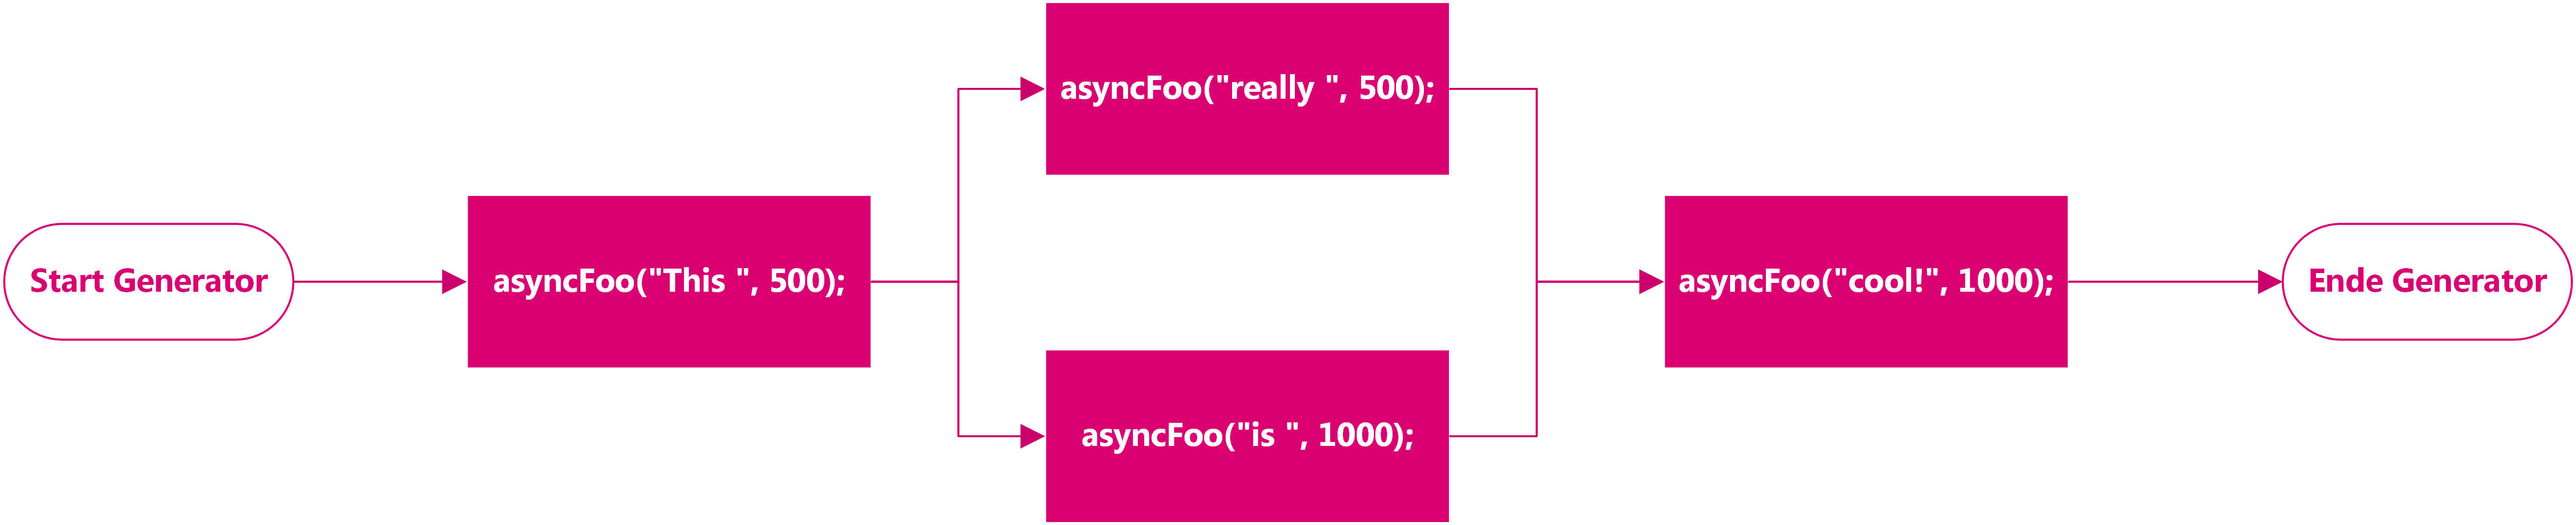
\includegraphics[width=1.0 \textwidth]{Images/generatorFlow.png}
			\caption[Abhängigkeiten asynchroner Aufrufe im Generator]{\label{generatorFlow}Die Abhängigkeiten der asynchronen Aufrufe im Generator aus Listing {\ref{snippets/asyncGenerator.js}}}.
		\end{figure}
		
		In diesem Beispiel wird deutlich, dass man unter Zuhilfenahme von Generators asynchronen Code sehr übersichtlich strukturieren kann. Er lässt sich genauso einfach aufschreiben und verstehen wie synchroner Code, ohne dabei auf die Vorteile der asynchronen Programmierung zu verzichten. Sogar die Fehlerbehandlung lässt sich innerhalb des Generators über den eigentlich synchronen \textsf{try-catch-finally}-Mechanismus realisieren. 
	
		\paragraph{Exkurs: \textsf{async-await} in künftigen Versionen von {ECMA\-Script}}
	
		Die durch die vorgestellte Benutzung von Generators  für asynchronen Code  erreichten Verbesserungen werden aktuell in der JavaScript Community als so wichtig erachtet, dass dieses Konzept in kommenden Versionen des ECMAScript Sprachstandards noch erweitert werden soll. Konkret sollen neue Schlüsselwörter \textsf{async} und \textsf{await} eingeführt werden, welche die Definition von speziellen Funktionen erlauben, die ähnlich ablaufen wie die oben gezeigten Generators mit externer Hilfsfunktion.
		
		In Zukunft wird es möglich sein, solche Funktionen direkt zu definieren, ohne einen Generator von einer Hilfsfunktion ausführen zu lassen. Die Sequenz von asynchronen Aufrufen lässt sich dann in eine \textsf{async}-Funktion schreiben, die direkt aufgerufen werden kann.
		
		\insertcode{snippets/asyncAwaitExample.js}{Die gleiche Sequenz wie in Listing~{\ref{snippets/asyncGenerator.js}}, jedoch mit \textsf{async-await} anstelle einer Hilfsfunktion zur Ausführung}
		
		Diese neue Syntax hat es zwar noch nicht in die neueste Version ECMAScript 7 (vgl.~\citep{EcmaTC39.2016}) geschafft, jedoch kann diese neue Syntax in bestimmten Laufzeitumgebungen wie z. B. Node.js ab Version 7.1 schon ausgeführt werden.\footnote{Einen guten Überblick über die in Node.js unterstützten Features liefert laufend aktualisiert \url{http://node.green}.}	
	
	
\section{Bewertung der neuen Sprachmittel}
	Aufgrund der großen Bedeutung asynchroner Programmierung in JavaScript sind die beiden vorgestellten Sprachmittel der Promises und Generators ein wichtiger Schritt für die Sprachentwicklung. Sie ermöglichen es, deutlich besser lesbaren und damit besser wartbaren Code zu schreiben als dies mit traditionellen Callbacks der Fall war. Auch werden die Probleme gelöst, die durch das Herausreichen der eigenen Programm-Continuation an fremden Code hervorgerufen wurden.
	
	Durch diesen offensichtlichen Zugewinn an Sicherheit und die einfachere Anwendung kann die Einführung dieser modernen Methoden in ECMAScript~6 rundweg positiv beurteilt werden. Sie sind ein wichtiger Baustein weiterhin komplexe JavaScript Anwendungen sowohl auf dem Server als auch im Client zu realisieren.
	
	Leider gibt es aber immer noch eine große installierte Basis an JavaScript Laufzeitumgebungen, die diese modernen Methoden nicht unterstützen.\footnote{Stellvertretend sei hier der Microsoft Internet Explorer genannt. Zur Kompatibilität von Laufzeitumgebungen zu verschiedenen Versionen des Standards siehe \url{https://kangax.github.io/compat-table/es6/}}

	Ist es trotzdem sinnvoll auf die neuen Sprachstandards und Methoden zu setzen?
	

	\paragraph{Promises} Für im Browser laufende Webanwendungen ist es wichtig, dass auch ältere Browser unterstützt werden um ein breites Publikum zu erreichen.
	Hier hat die Programmiererin keine Kontrolle über die Laufzeitumgebung und kann sich daher nicht auf die Kompatibilität zum ECMAScript~6 Standard verlassen.
	
	Trotzdem spricht nichts gegen die Verwendung von Promises: Promises können sehr leicht als Polyfill in älteren Laufzeitumgebungen von JavaScript nachgerüstet werden. Damit ist es möglich die inzwischen standardisierten Features auch dort zu nutzen und von den Verbesserungen zu profitieren. Es muss lediglich eine passende Polyfill-Bibliothek mit ausgeliefert werden. 
	
	Sogar ältere APIs, welche mit Callbacks nach dem Error-First-Pro"-to"-koll und einem trailing Callback arbeiten, lassen sich leicht per \textsf{promisify()} in eine äquivalente API umsetzen, die Promises statt Callbacks nutzt.\footnote{Details dazu finden sich im Anhang \ref{promisify}.}
	
	
	\paragraph{Generators} Mit Generators wurde eine neue Syntax in Java"-Script eingeführt, die sich nicht einfach über Bibliotheksfunktionen nachrüsten lässt. 
	
	Wenn man die Laufzeitumgebung unter Kontrolle hat, wie es bei serverseitigen Applikationen üblicherweise der Fall ist, so kann das Konzept der Generators für asynchrone Control-Flows auf jeden Fall genutzt werden. 
	
	Der Einsatz von Generators in Webanwendungen sollte dagegen für den Einzelfall abgewogen werden: Programme, die Generators verwenden und auch in älteren Laufzeitumgebungen vor ECMAScript~6 laufen sollen, müssen  vorher in kompatiblen Code transpiliert werden.\footnote{Unter Transpilation versteht man die Übersetzung von einer Quellsprache in eine andere Quellsprache. In diesem Fall also von ECMAScript~6 in ECMAScript~5, welches von allen aktuellen Browsern unterstützt wird. (vgl.~\citep{Sengstacke.2016})}
	
	Es ist im Einzelfall zu prüfen, ob der Gewinn durch die Verwendung von Generators den zusätzlichen Build-Step rechtfertigt. Wenn aber vor der Veröffentlichung einer Webanwendung sowieso diverse Build-Steps notwendig sind, ist es in der Regel kein Problem, einen solchen Transpile-Step einzufügen. Der maschinell erzeugte Code ist aber nicht mehr gut lesbar und daher schwerer zu debuggen.
	Wenn sowieso ein Transpile-Schritt eingefügt wird, dann sollte man gleich den Schritt zu \textsf{async-await} gehen, da der Code dadurch noch prägnanter wird.
	
	\subsection*{Fazit}
	
		Schlecht lesbarer Code ist im Umfeld von asynchroner Programmierung häufig anzutreffen. Die "`Callback Hell"' ist allgegenwärtig.
		
		Durch die neuen Sprachmittel von ECMAScript~6 wurden jedoch Möglichkeiten geschaffen, auch asynchronen Code lesbar aufzuschreiben und vertrauenswürdig auszuführen. Dabei muss nicht auf die Vorteile der asynchronen Programmierung verzichtet werden.
		
		\begin{figure}[h]\label{xkcdCodeQuality2}\centering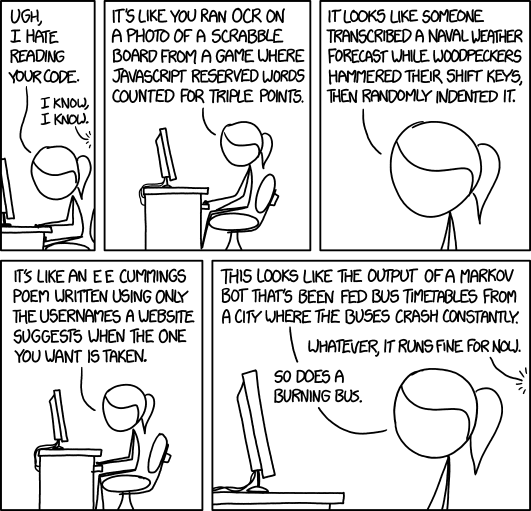
\includegraphics[width=0.55 \textwidth]{Images/code_quality_2.png}\caption[xkcd: Code Quality 2]{xkcd: Code Quality 2~(aus \citep[]{Munroe.2016})}
			
		\end{figure}
		
		Die vorgestellten modernen Methoden, die ECMAScript~6 für die asynchrone Programmierung bietet, sind daher ein wichtiger Meilenstein, um große Applikationen sicher und effizient zu entwickeln und zu warten.
		
		Es gibt spätestens seit der Einführung des ECMAScript~6 Standards keine Entschuldigung mehr für asynchronen Spaghetti-Code, wie dies noch 2007 in "`Web Applications -- Spaghetti Code for the 21st Century"'~\citep{Mikkonen.2007} beklagt wurde. JavaScript bietet heutzutage alle Möglichkeiten, gut strukturierten, effizienten asynchronen Code zu schreiben. Es ist an den Programmiererinnen diese Möglichkeiten zu nutzen und dazu beizutragen, dass JavaScript sein traditionell schlechtes Image ablegen kann. 

%----------------------------------------------------------------------------------------
%	BIBLIOGRAPHY
%----------------------------------------------------------------------------------------

\cleardoublepage

\renewcommand{\refname}{\spacedlowsmallcaps{References}} % For modifying the bibliography heading

\renewcommand{\refname}{Literatur} 

\bibliographystyle{dinat}

\bibliography{literatur} % The file containing the bibliography

%----------------------------------------------------------------------------------------

\cleardoublepage

\appendix

\newcommand{\appendixpagenumbering}{
	\break
	\pagenumbering{arabic}
	\renewcommand{\thepage}{\thesection-\arabic{page}}
}

\appendixpagenumbering

\counterwithin{figure}{section}
\counterwithin{lstlisting}{section}

\section{Muster der asynchronen Programmierung in ECMAScript 6}

	In diesem Anhang sollen einige typische Muster der asynchronen Programmierung in ECMAScript~6 inklusive Code-Beispielen vorgestellt werden. Diese Beispiele sollen nicht der ausführlichen Diskussion der Konzepte dienen, sie sind vielmehr als Referenz und Anregung für eigene Projekte gedacht, in denen die neuen Sprachfeatures von ECMA"-Script~6 eingesetzt werden sollen. Für einen solchen Einsatz sind Anpassungen und Ergänzungen unumgänglich. Vor dem produktiven Einsatz sollte daher auf jeden Fall die umfangreich im Netz vorhandene Dokumentation herangezogen werden. 
	
	Auch bei der Programmierung in JavaScript gilt es den Bibliotheksgedanken zu leben und lieber etwas mehr Zeit in die Suche nach einer passenden Bibliotheksfunktion zu investieren als eine Funktion selber neu zu implementieren.
	
	\begin{quote}Jede nicht selbst geschriebene Programmzeile ist ein Gewinn, jede Implementierung einer noch so kleinen Funktion, die es bereits in irgendeiner Bibliothek gibt, ist ein Verlust.~\citep[S.~333]{Steimann.2010}\end{quote}
	
	Gerade bei der Programmierung mit Node.js wird der Programmiererin die Benutzung von ausgereiften und getesteten Bibliotheksfunktionen leicht gemacht, da es mit \textsf{npm} (siehe \url{https://www.npmjs.com/}) ein hervorragend gepflegtes und extrem umfangreiches Paketverwaltungssystem gibt. Eine Suche nach Bibliotheksfunktionen auf \textsf{npm} ist meistens von Erfolg gekrönt. Sollte  es einmal kein passendes Paket dort geben, so ist die Programmiererin ermuntert, die eigene Implementierung dort für andere User zugänglich zu machen.
	
	\skippingparagraph
	In den nächsten Abschnitten sollen Beispiele zu diesen Themen gegeben werden:
	\begin{itemize}[nosep]
		\item Umwandlung traditioneller Callback-APIs in Funktionen, die eine Promise zurückgeben
		\item Error Handling in Promise Chains
		\item asynchrone Sequenzen mit verschiedenen Parametern
		\item asynchrone Funktionen mit Timeout
		\item Zusammensetzen komplexer Abläufe -- "`functional composition"'
	\end{itemize}
	
	\subsection{\label{promisify}Anpassung älterer APIs an Promises}
	
		Obwohl die Benutzung von Promises sich für asynchrone Aufrufe immer mehr durchsetzt, sind in der JavaScript Welt noch sehr viele Bibliotheken verfügbar und gebräuchlich, die ihre Ergebnisse nach dem traditionellen Callback-Verfahren liefern. Um auch solche Funktionen mit den neuen Mechanismen nutzen zu können, muss die asynchrone Funktion, die einen Callback zur Rückgabe des Ergebnisses erwartet, in eine Funktion umgewandelt werden, die statt dessen eine Promise zurückliefert.
		
		Dieser Vorgang wird häufig als "`Promisification"' oder "`Lifting"' bezeichnet. Durch den ECMAScript~6 Standard wird dieser Vorgang nicht direkt spezifiziert, aber es existieren viele externe Bibliotheken die entsprechende Funktionen bieten. Diese können problemlos auch im Zusammenspiel mit ES6-Promises genutzt werden.\footnote{Siehe z. B. das Paket \url{https://www.npmjs.com/package/es6-promisify} oder die Funktionen in der Bluebird Promise-Library \url{http://bluebirdjs.com/docs/api/promisification.html}. Eine Suche nach dem Stichwort "`promisify"' auf \textsf{npm} liefert aktuell 380 Ergebnisse (\url{https://www.npmjs.com/search?q=promisify}).}
		
		Auch wenn es angesichts der ausreichend vorhandenen fertigen Lösungen nicht notwendig sein sollte ein solches Lifting selber zu implementieren, so soll doch der Vorgang an einem Stück Beispielcode gezeigt werden. Das Beispiel in Listing \ref{snippets/promisory.js} folgt weitgehend der Erklärung in \cite[S.~76]{Simpson.2015}.
		
		\insertcode{snippets/promisory.js}{[Wrapper Funktion zur Umwandlung von Callback APIs in Promise APIs]{Wrapper Funktion zur Umwandlung von Callback APIs in Promise APIs (aus \citep[S.~76]{Simpson.2015})}}
		
		Der angegebene Code erweitert den Prototyp \textsf{Promise} um eine Methode \textsf{wrap()}, welche eine Funktion erwartet, die den Konventionen Error-First und Trailing-Callback folgt. Als Rückgabe erhält die Programmiererin eine neue Funktion, die keinen Callback mehr erwartet, sondern anstelle dessen eine Promise zurückliefert. Diese \emph{settled} im Status \emph{fullfilled} wenn der zugrundeliegende Aufruf erfolgreich war und im Status \emph{rejected} wenn ein Fehler auftrat.
		
		Die Anwendung des Wrappers wird in Listing \ref{snippets/promisifiedFoo.js} gezeigt. Die Funktion \textsf{foo} ruft eine asynchrone Funktion auf, die einen Callback erwartet. Zunächst wird \textsf{foo} mit traditionellem Callback verwendet und dann mittels des vorgestellten Wrappers in eine Funktion \textsf{fooPromise} verwandelt und über ihr Promise-API verwendet.
		
		\insertcode{snippets/promisifiedFoo.js}{Verwendung des Promisification Wrappers}.
	
	\subsection{Error Handling in Promise Chains}
	
		Um die vielfältigen Möglichkeiten der struktutrierten Fehlerbehandlung bei der Verwendung von Promises zu verdeutlichen, soll in diesem Abschnitt ein etwas umfangreicheres Beispiel angegeben werden. Dabei werden verschiedenen Methoden zur Fehlerbehandlung gezeigt, die in der Praxis vielfältig kombiniert werden.
	
		Ein Rejection-Handler muss nicht zwangsläufig am Ende einer Pro\-mise Chain benutzt werden, sondern kann auch in der Mitte einer Kette installiert werden, um zum Beispiel detailliertere Log-Dateien zu schreiben oder frühzeitig nicht mehr benötigte Resourcen freizugeben. 
		
		Dabei ist jedoch zu beachten, dass die vom Rejection-Handler zurückgegebene Promise nicht automatisch den Status \emph{rejected} annimmt. 
		Mit einem in der Mitte der Promise Chain eingehängten Rejection-Handler kann also die weitere Abarbeitung wieder aufgenommen werden. Wenn man die Abarbeitung nach einem Fehler jedoch endgültig abbrechen möchte, so muss man aus dem Rejection-Handler wieder eine \emph{rejected} Promise zurückgeben. Dazu ist es häufig zweckmäßig, den empfangenen Rejection Reason wieder als Exception zu werfen und damit die vom Rejection-Handler zurückgegebene Promise ihrerseits zurück zu weisen.
		
		\insertcode{snippets/promiseChainRejectionHandler_2.js}{Mehrere Rejection-Handler inmitten einer Promise-Chain}
		
		Am Beispiel in Listing \ref{snippets/promiseChainRejectionHandler_2.js} werden die verschiedenen Möglichkeiten verdeutlicht:
		Für eine normale Ausführung sollen die asynchronen Funktionen \textsf{bar}, \textsf{baz} und \textsf{booze} jeweils mit dem Resultat ihrer Vorgängerfunktion aufgerufen werden. Es wird angenommen, dass bei einem Fehlschlag der Funktion \textsf{bar} mit einem default Wert weiter gearbeitet werden kann. Bei Fehlschlagen von \textsf{baz} jedoch soll die Abarbeitung der Kette abgebrochen werden, jedoch muss in diesem Fall aufgeräumt werden. Fehlschlagen von \textsf{booze} erfordert keine spezielle Fehlerreaktion.
		
		Es wird also hinter \textsf{bar} ein Rejection-Handler in die Promise-Chain eingehängt. Dieser liefert bei Fehlschlag eine \emph{fulfilled} Promise mit default Wert. Der nächste Rejection-Handler hinter \textsf{baz} muss neben dem Aufräumen auch dafür sorgen, dass die Kette nicht weiter abgearbeitet wird. Daher wird der Eingangsfehler aus dem Aufruf von \textsf{baz} in die Rückgabepromise des Rejection-Handlers verpackt. Diese \emph{rejected} Pro"-mise wird nun bis zum finalen Rejection-Handler durch die Kette gereicht.
		
		Die geneigte Leserin mag sich selber überlegen, wie die beschriebene Logik mittels konventioneller Callbacks zu formulieren wäre.
	

	\subsection{Asynchrone Sequenz mit verschiedenen Parametern}
		
	Zuweilen kommt es vor, dass eine bestimmte Sequenz aus asynchronen Aufrufen nacheinander abgearbeitet werden soll. Die auszuführende asynchrone Funktion ist dabei immer die gleiche, allerdings sind nacheinander unterschiedliche Parameter an diese zu übergeben. Dieses Muster kommt relativ häufig beim Schreiben von Tests vor. Die zu testende Funktion soll nacheinander mit verschiedenen Parametern aufgerufen werden. Bei einem auftretenden Fehler soll die gesamte Aufrufkette abgebrochen werden.
	
	Im folgenden Beispiel soll die Funktion getestet werden, die eine Web-API zum Hinzufügen weiterer Teilnehmer zur Verfügung stellt. Je nachdem, welche Vorgeschichte der aktuelle Testfall hat, soll die zu testende Funktion entweder den Status 200 ("`OK"') oder den Status 409 ("`Conflict"') zurück melden. Alle Ergebnisse der sequentiellen Aufrufe sollen bei Erfolg in einem Array zur Verfügung stehen. 
	
	Es wäre einfach den Testfall manuell als Promise-Chain zu formulieren. Übersichtlicher ist es jedoch, sich eine kleine Hilfsfunktion zu schreiben, welche die Aufrufsequenz übernimmt und die Parameter aus einer generischen Kollektion entnimmt.
	
	Eine solche Hilfsfunktion ist in Listing \ref{snippets/promiseSequence.js} dargestellt:
	
	\insertcode{snippets/promiseSequence.js}{[Hilfsfunktion, \textsf{sequence} zum sequentiellen Aufruf einer asynchronen Funktion mit verschiedenen Parametern]{Hilfsfunktion  \textsf{sequence} zum sequentiellen Aufruf einer asynchronen Funktion mit verschiedenen Parametern. (aus \citep[S.~33]{Parker.2015})}}
	
	Die interne Hilfsfunktion \textsf{chain()} wird beginnend mit dem ersten Parameter im \textsf{.then()} der vorherigen Promise immer wieder rekursiv aufgerufen, bis das Parameter-Array erschöpft ist. Dann werden die Ergebnisse der einzelnen Aufrufe als Array in einer Promise verpackt zurückgegeben. 
	
	Interessant bei diesem Muster ist der rekursive Aufruf der \textsf{chain()}-Funktion: Trotz der Rekursion kann hier kein Stack-Overflow auftreten, da die rekursiven Aufrufe nicht direkt erfolgen, sondern asynchron in die Queue des Laufzeitsystems eingereiht werden. Jeder neue Aufruf startet daher wieder mit einem leeren Stack.
	
	Im folgenden Listing \ref{snippets/promiseSequenceUsage.js} wird ein Testfall eines Unit-Tests simuliert, der sich die vorgestellte \textsf{sequence()}-Funktion zu nutze macht, um nacheinander mehrere Testfälle auf der Funktion \textsf{addParticipantPost} auszuführen.
	
	\insertcode{snippets/promiseSequenceUsage.js}{Simulierter Testfall unter Verwendung von \textsf{sequence}.}

	\subsection{Asynchrone Funktionen mit Timeout}
	
	Häufig ist es sinnvoll den Aufruf von asynchronen Funktionen mit einem Timeout zu versehen. Dadurch kann garantiert werden, dass nach Ablauf der festgelegten Zeit auch tatsächlich ein Ergebnis vorliegt. Dieses kann dann zwar auch ein Fehler oder ein Default-Wert sein, jedoch ist es garantiert vorhanden und die eigene Applikation kann geeignete Maßnahmen ergreifen.
	
	Mit \textsf{Promise.race()} lässt sich sehr einfach eine Hilfsfunktion erstellen, die einen asynchronen Funktionsaufruf mit einem Timeout versieht. Optional kann ein Default-Wert angegeben werden. Eine Möglichkeit einer solchen Hilfsfunktion ist in Listing \ref{snippets/timeoutPromise.js} angegeben.
	
	\insertcode{snippets/timeoutPromise.js}{Hilfsfunktion, um einen asynchronen Aufruf mit einem Timeout und einem optionalen Default-Wert zu versehen}
	
	Der Funktion wird als erster Parameter die Promise aus einem asynchronen Aufruf übergeben. Im zweiten Parameter wird ein Timeout in Millisekunden spezifiziert. Der dritte Parameter ist optional und gibt einen Default-Wert an. Wenn die übergebene Promise nach der angegebenen Zeit noch nicht \emph{settled} ist, dann wird die resultierende Promise entweder mit einem timeout-Fehler \emph{rejected} oder aber mit dem angegebenen Default-Wert \emph{fulfilled}.
	Ein Anwendungsbeispiel ist in Listing \ref{snippets/timeoutPromiseUsage.js} zu sehen.
	
	\insertcode{snippets/timeoutPromiseUsage.js}{Anwendung einer Promise mit Timeout und Default-Wert}
	
	Auch in diesem Fall ist es sinnvoll, eine solche Funktion nicht selber zu implementieren sondern geeignete Bibliotheksfunktionen einzubinden. In diesem Fall lohnt sich ein Blick auf \url{https://www.npmjs.com/package/time-limit-promise}.
	
	
	
	\subsection{Pipelining komplexer Abläufe -- "`functional composition"'}
	
	Ein bekanntes Muster der Software-Architektur ist das "`Pipe-and-Filter"' Muster, bei dem komplexe Aufgaben derart in kleinere Teilaufgaben zerlegt werden, dass diese Teilaufgaben einzeln einfach zu realisieren sind. Auf die Daten werden nacheinander einzelne Filter angewendet und das Ergebnis über eine Pipe an die nächste Filterstufe weiter transportiert.
	
	Ganz ähnlich kann man sich eine Sequenz aus asynchronen und synchronen Funktionen vorstellen, die einen Eingangswert durch mehrere hintereinander angewendete Filterstufen in ein Endergebnis transformiert. Das Ergebnis einer Stufe ist jeweils das Eingangsdatum der nächsten Stufe. Dadurch lassen sich über die Komposition einfacher Funktionen komplexe Abläufe realisieren. Man spricht daher auch von "`functional composition"'.
	
	Da Funktionen in JavaScript First-Class-Citizens sind, können sie leicht in einem Array gespeichert werden. Im folgenden Listing \ref{snippets/promisePipeline.js} wird eine Hilfsfunktion vorgestellt, die in einem Array abgelegte Funktionen nacheinander aufruft und jeweils das Ergebnis der vorhergehenden Funktion als Eingangsparameter für die nachfolgende Funktion verwendet. Es wird eine Pipeline aufgebaut, um eine komplexe Funktion aus einfachen Bestandteilen zusammen zu setzen.
	
	\insertcode{snippets/promisePipeline.js}{[Hilfsfunktion zum Pipelining]{Hilfsfunktion zum Pipelining (aus~\citep{Harrington.2015})}}
		
	
	Es wird ein Pipeline-Konstruktor exportiert, dem zur Erzeugung eines neuen Objekts ein Array aus Funktionen übergeben wird. Dieses Pipeline-Objekt hat eine Methode \textsf{go()}, welche ihre eigenen Parameter an die erste Funktion des Arrays übergibt und darauffolgend das Ergebnis eines jeden Funktionsaufrufs als Eingangsparameter des jeweils nächsten benutzt. Wenn das übergebene Funktionsarray erschöpft ist wird das Endergebnis zurückgegeben. Bei dem Array mit den einzelnen Funktionen ist es egal, ob diese asynchron eine Promise zurückgeben, oder direkt synchron ein Ergebnis. Alle Aufrufe werden über eine Promise-Chain asynchron entkoppelt.
	
	Die Anwendung der vorgestellten Funktion wird im Listing \ref{snippets/promisePiplineUsage.js} anhand eines simplen Workflows demonstriert. Es lassen sich natürlich auch leicht sinnvollere Anwendungen dieses Musters finden.
	
	\insertcode{snippets/promisePiplineUsage.js}{Anwendung einer Funktionspipeline zur Realisierung eines komplexen Workflows}
	
	Es soll nicht unerwähnt bleiben, dass es natürlich auch für das hier vorgestellte Muster schon vielfältige Realisierungen als Bibliotheksfunktionen gibt. Aus der Masse sticht hier die Realisierung mittels der Bibliothek "`Ramda"' hervor, die sich auf die funktionale Programmierung in JavaScript spezialisiert hat und dadurch häufig sehr elegante Lösungen für ansonsten relativ komplizierte Abläufe bietet. Siehe hierzu: \url{http://ramdajs.com/docs/#pipeP}.
	
%	\subsection{Zwei-Wege-Kommunikation in Generators}
%	
%		Alle Fälle der Zwei-Wege Kommunikation sind im Listing \ref{snippets/incrementGenerator.js} zu sehen.
%		
%		\insertcode{snippets/incrementGenerator.js}{Von außen mittels \textsf{it.next(value)}, \textsf{it.return(value)} und \textsf{it.throw(e)} gesteuerter Generator.}
%		
%		Im gezeigten Beispiel wird ein Generator definiert, der als Startparameter bei der Erzeugung des \emph{Iterators} einen Startwert und eine Schrittweite als Parameter bekommt. Er liefert in jedem Durchlauf den um die Schrittweite erhöhten Wert. Die Schrittweite kann von außen über \textsf{it.next(step)} beeinflusst werden. Der von außen eingespeiste Wert wird bei der Wiederaufnahme nach einer Pause am \textsf{yield} Statement übernommen. Zu beachten ist, dass beim ersten Aufruf \textsf{it1.next(666)} der Parameter ignoriert wird. Die Parameterübernahme findet nur statt, wenn der \emph{Generator} seine Bearbeitung nach einer Wertanfrage durch einen \emph{Iterator} wieder aufnimmt. Das ist beim ersten Aufruf von \textsf{it.next()} nicht der Fall und daher findet auch keine Wertübernahme statt.(vgl.~\citep[S.~84]{Simpson.2015})\todoInfo{Das sollte eigentlich auch aus der Spezifikation §25.3.3.3 rauskommen. Sehe ich aber nicht direkt. sieh nochmal bei Kyle nach.}
%		
%		Im ersten Beispielablauf wird der Generator durch den Aufruf von \textsf{it.return(42)} beendet und liefert als Ergebnis \textsf{\{ value: 42, done: true \}}. Im zweiten Beispielablauf wird der \emph{Generator} durch eine von außen injizierte Exception beendet, die innerhalb des \emph{Generators} nicht behandelt wird. Sie wird also wieder nach außen geworfen und muss dort gefangen werden.


\end{document}